% указываем класс документа
\documentclass[12pt,a4paper,openany]{extarticle}
% подключаем собственный стилевой файл 
\usepackage{mystyle}
% указываем язык (для автоматической вставки слов, типа "Глава", "Содержание", "Литература", "рис." и пр.
\selectlanguage{russian}

\usepackage{listings}
\usepackage{color}

\definecolor{dkgreen}{rgb}{0,0.6,0}
\definecolor{gray}{rgb}{0.5,0.5,0.5}
\definecolor{mauve}{rgb}{0.58,0,0.82}

\lstset{frame=tb,
	language=Python,
	aboveskip=3mm,
	belowskip=3mm,
	showstringspaces=false,
	columns=flexible,
	basicstyle={\small\ttfamily},
	numbers=none,
	numberstyle=\tiny\color{gray},
	keywordstyle=\color{blue},
	commentstyle=\color{dkgreen},
	stringstyle=\color{mauve},
	breaklines=true,
	breakatwhitespace=true,
	tabsize=3
}

\begin{document}

\part*{Лабораторная работа №3\\
Управление мотором EV3}

\section{Методические рекомендации}
\hspace*{\parindent}До начала работы студент должен выполнить предыдущие лабораторные этого цикла.

\section{Теоретические сведения}
\hspace*{\parindent}В~данной работе мы познакомимся с одной из самых простых стратегий управления, которая носит название \textit{П-регулятор}.
Объяснение ее сути предлагаем привести на конкретном примере.
Для этого представим, что перед нами стоит задача написать для блока EV3 такую программу-алгоритм, которая бы запускала мотор на вращение вплоть до достижения его выходным валом заданного угла поворота, а потом фиксировала бы его в этом положении.

В~прошлых работах мы показали, что поведение исследуемых систем определяется характером управляющего воздействия.
Также мы выяснили, что таковым для нашего мотора является напряжение, подаваемое на него с блока EV3.
Из этого можно сделать вывод о том, что наша задача сводится к нахождению определенной зависимости $U_{ctrl}(t)$, которая и обеспечит нужное его поведение.

А~теперь с учетом сказанного покажем, как можно прийти к концепции П-регулятора путем простых логических умозаключений.

\paragraph*{П-регулятор}$\phantom{-}$\\
\hspace*{\parindent}Заметив из материалов прошлой работы, что между угловой скоростью вращения вала мотора и подаваемым на него напряжением существует прямая зависимость\lefteqn{,}\footnote{Под прямой зависимостью мы подразумеваем принцип <<чем больше напряжение, тем больше и скорость>>.
Это взаимосвязь между указанными величинами вытекает хотя бы из расчетной формулы для постоянной $k_e$.} в качестве первого варианта управляющей стратегии логично предложить следующую:
\begin{quote}
\textsl{Подавать максимальное (в таком случае желаемый угол будет достигнут быстрее) напряжение на мотор до тех пор, пока его вал не повернется на заданный угол.
Потом отключить напряжение.} 
\end{quote}
При этом график зависимости управляющего напряжения от текущего угла поворота вала примет вид, показанный на рис.~\ref{1_graph}, а ее аналитическое выражение запишется как
\begin{equation}
	U_{ctrl}(\theta) = 
	\left\{	
	\begin{aligned} 
		\!U_{ctrl}^{max}\!&, &&\theta < \theta_w; \\
		\!0&, &&\theta \geqslant \theta_w,
	\end{aligned}
	\right.	
\end{equation}
где $U_{ctrl}^{max}$~--- максимальное напряжение, которое может обеспечить источник энергии; $\theta_w$~--- угол, на который должен повернуться вал.

\begin{figure}[h]
	\noindent\centering{ 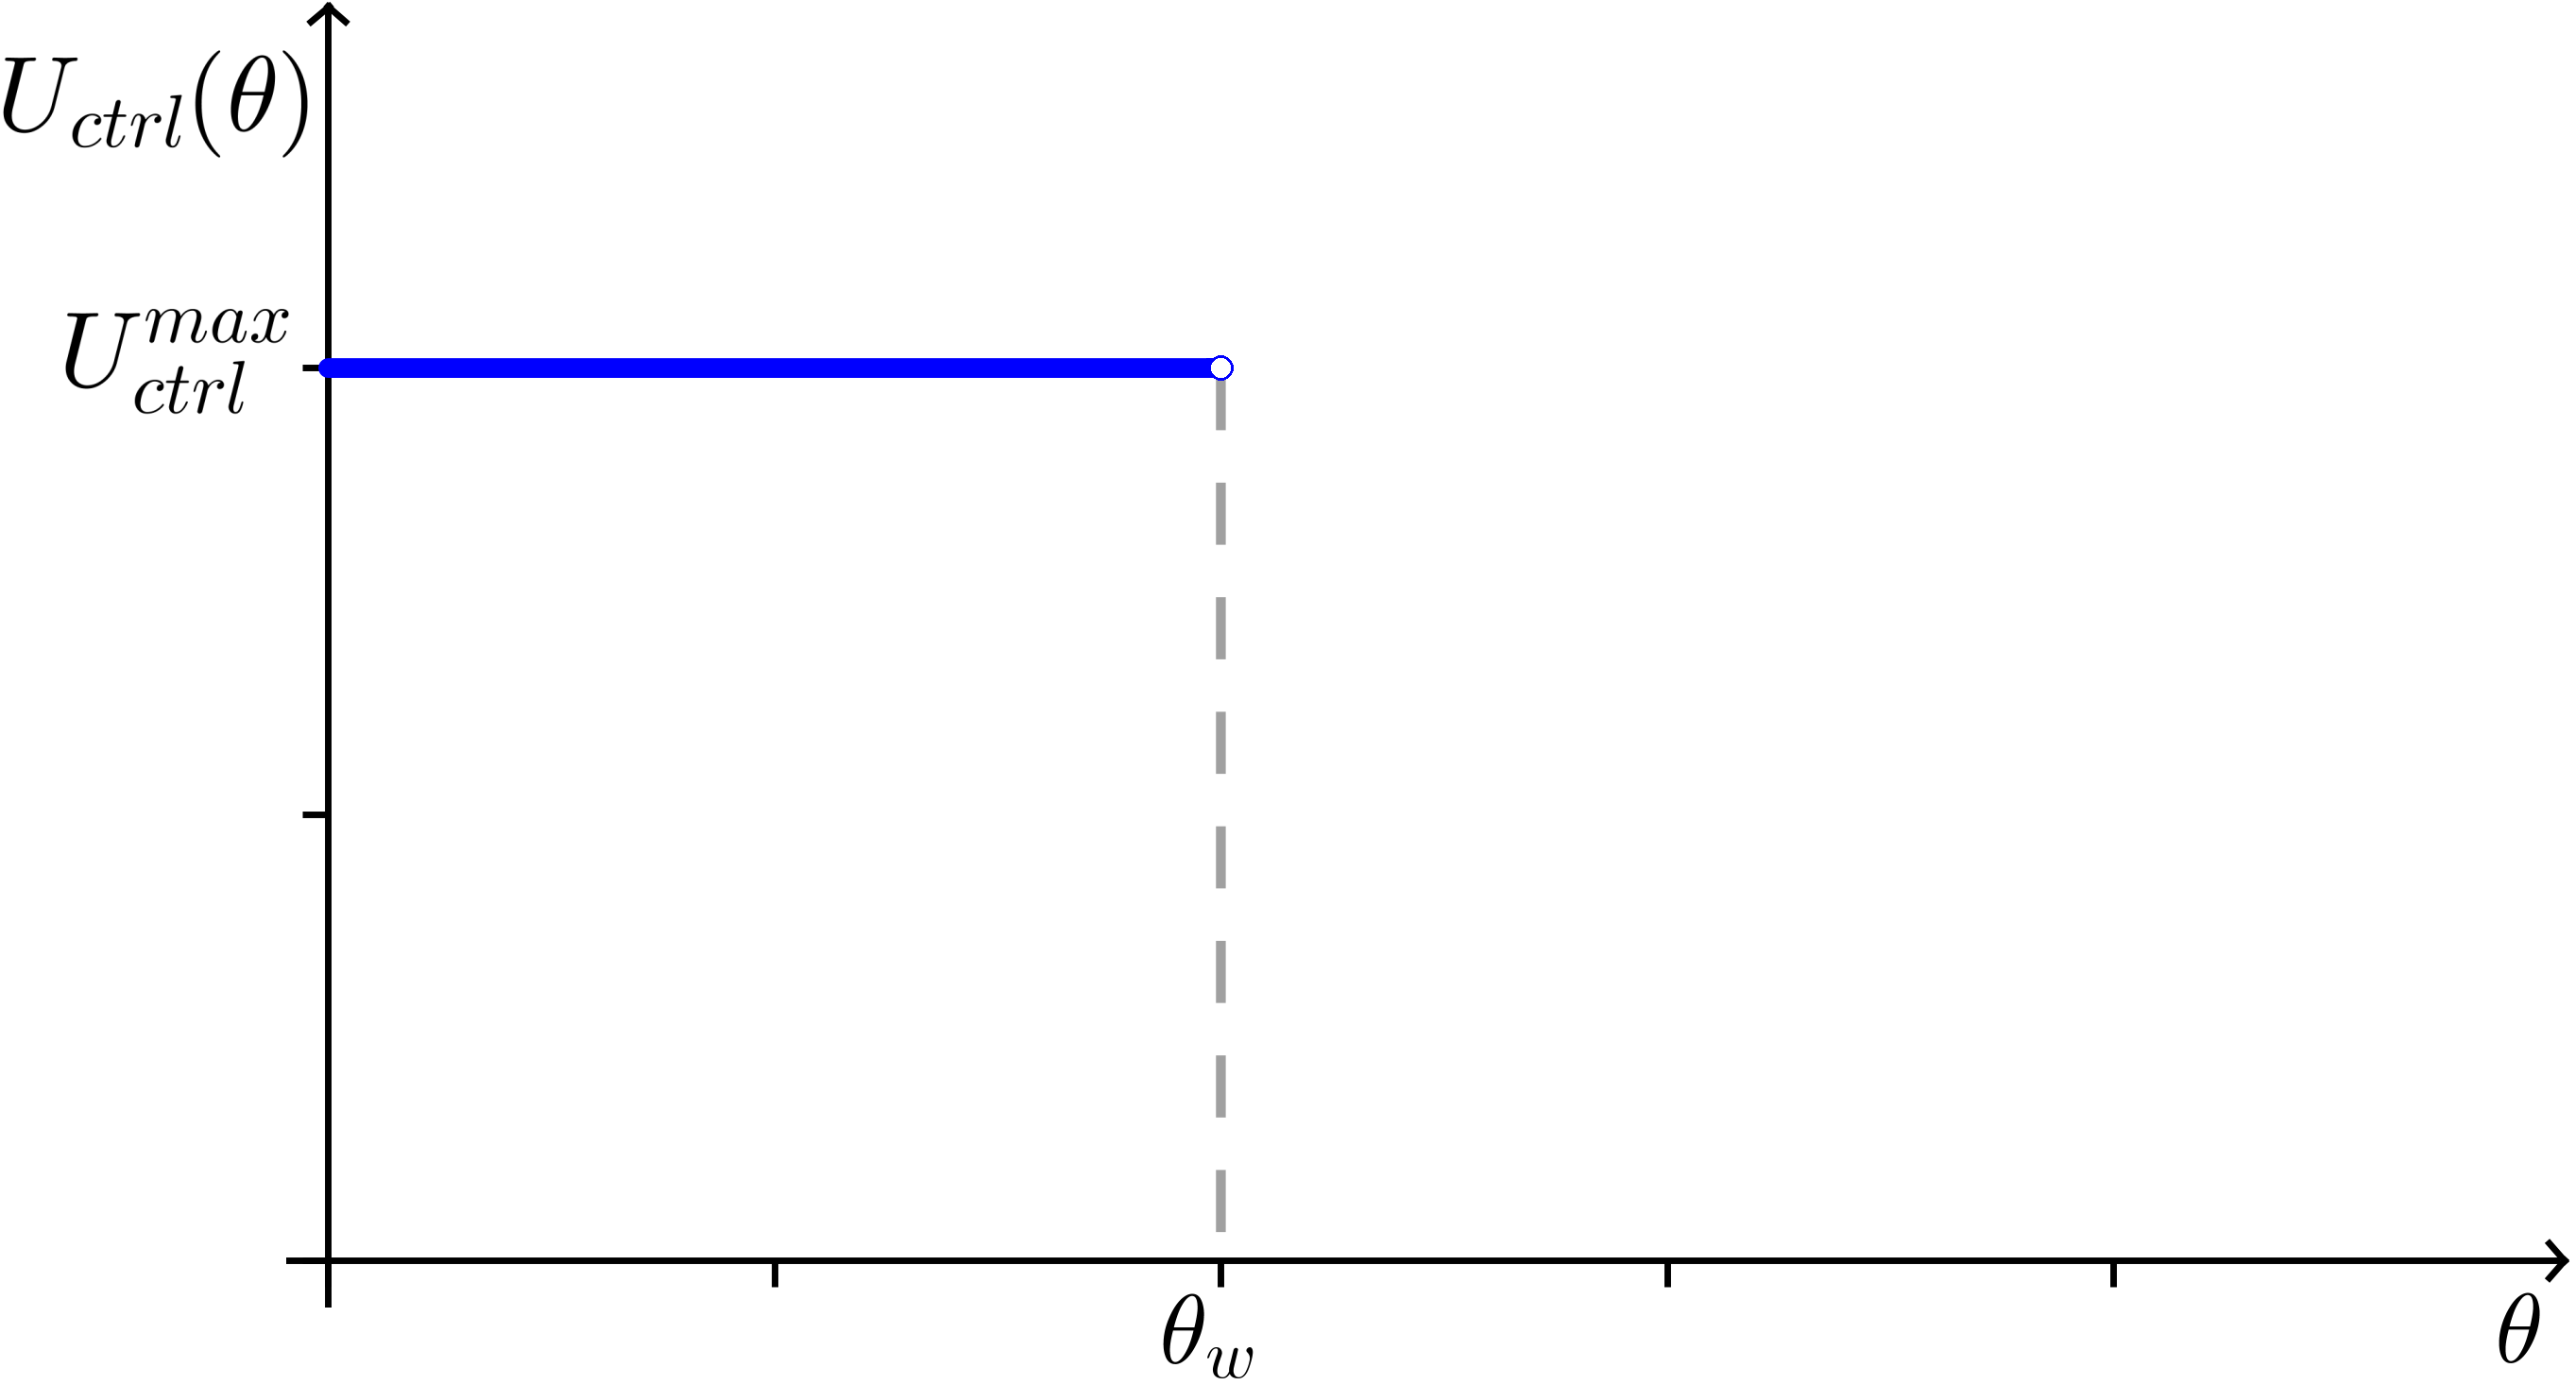
\includegraphics[scale=1]{1_graph.png} }
	\caption{График самой простой управляющей стратегии.}
	\label{1_graph}
\end{figure}

Данная стратегия обречена на провал, а причина этому~--- инерционность механического движения.
Вал мотора EV3, достигнув желаемого угла поворота, не останется в этом положении, а будет продолжать вращаться.
Спустя определенный промежуток времени он, конечно, остановится, но заслуга в этом будет принадлежать исключительно действующим на него силам сопротивления его движению, например силам трения.

Чтобы воспрепятствовать указанному перелету, логично добавить в управляющий алгоритм воздействие, которое бы тормозило вал при достижении им угла $\theta_w$ и возвращало его на место, если бы тот все-таки повернулся на угол, больший желаемого.
C~учетом этого новый вариант стратегии запишется в виде:
\begin{quote}
\textsl{Подавать максимальное напряжение на мотор до тех пор, пока его вал не повернется на заданный угол.
В случае перелета сменить полярность напряжения.
Повторять процесс до полной остановки вала.} 
\end{quote}
Записав ее в аналитическом виде, получим следующее выражение:
\begin{equation}
	U_{ctrl}(\theta) = 
	\left\{
	\begin{aligned}
		\!U_{ctrl}^{max}\!&, &&\theta < \theta_w; \\
		\!0&, &&\theta = \theta_w; \\		
		\!-U_{ctrl}^{max}\!&, &&\theta > \theta_w, 
	\end{aligned}
	\right.
\end{equation}
а построив график~--- ломаную, показанную на рис.~\ref{2_graph}.

\begin{figure}[h]
	\noindent\centering{ 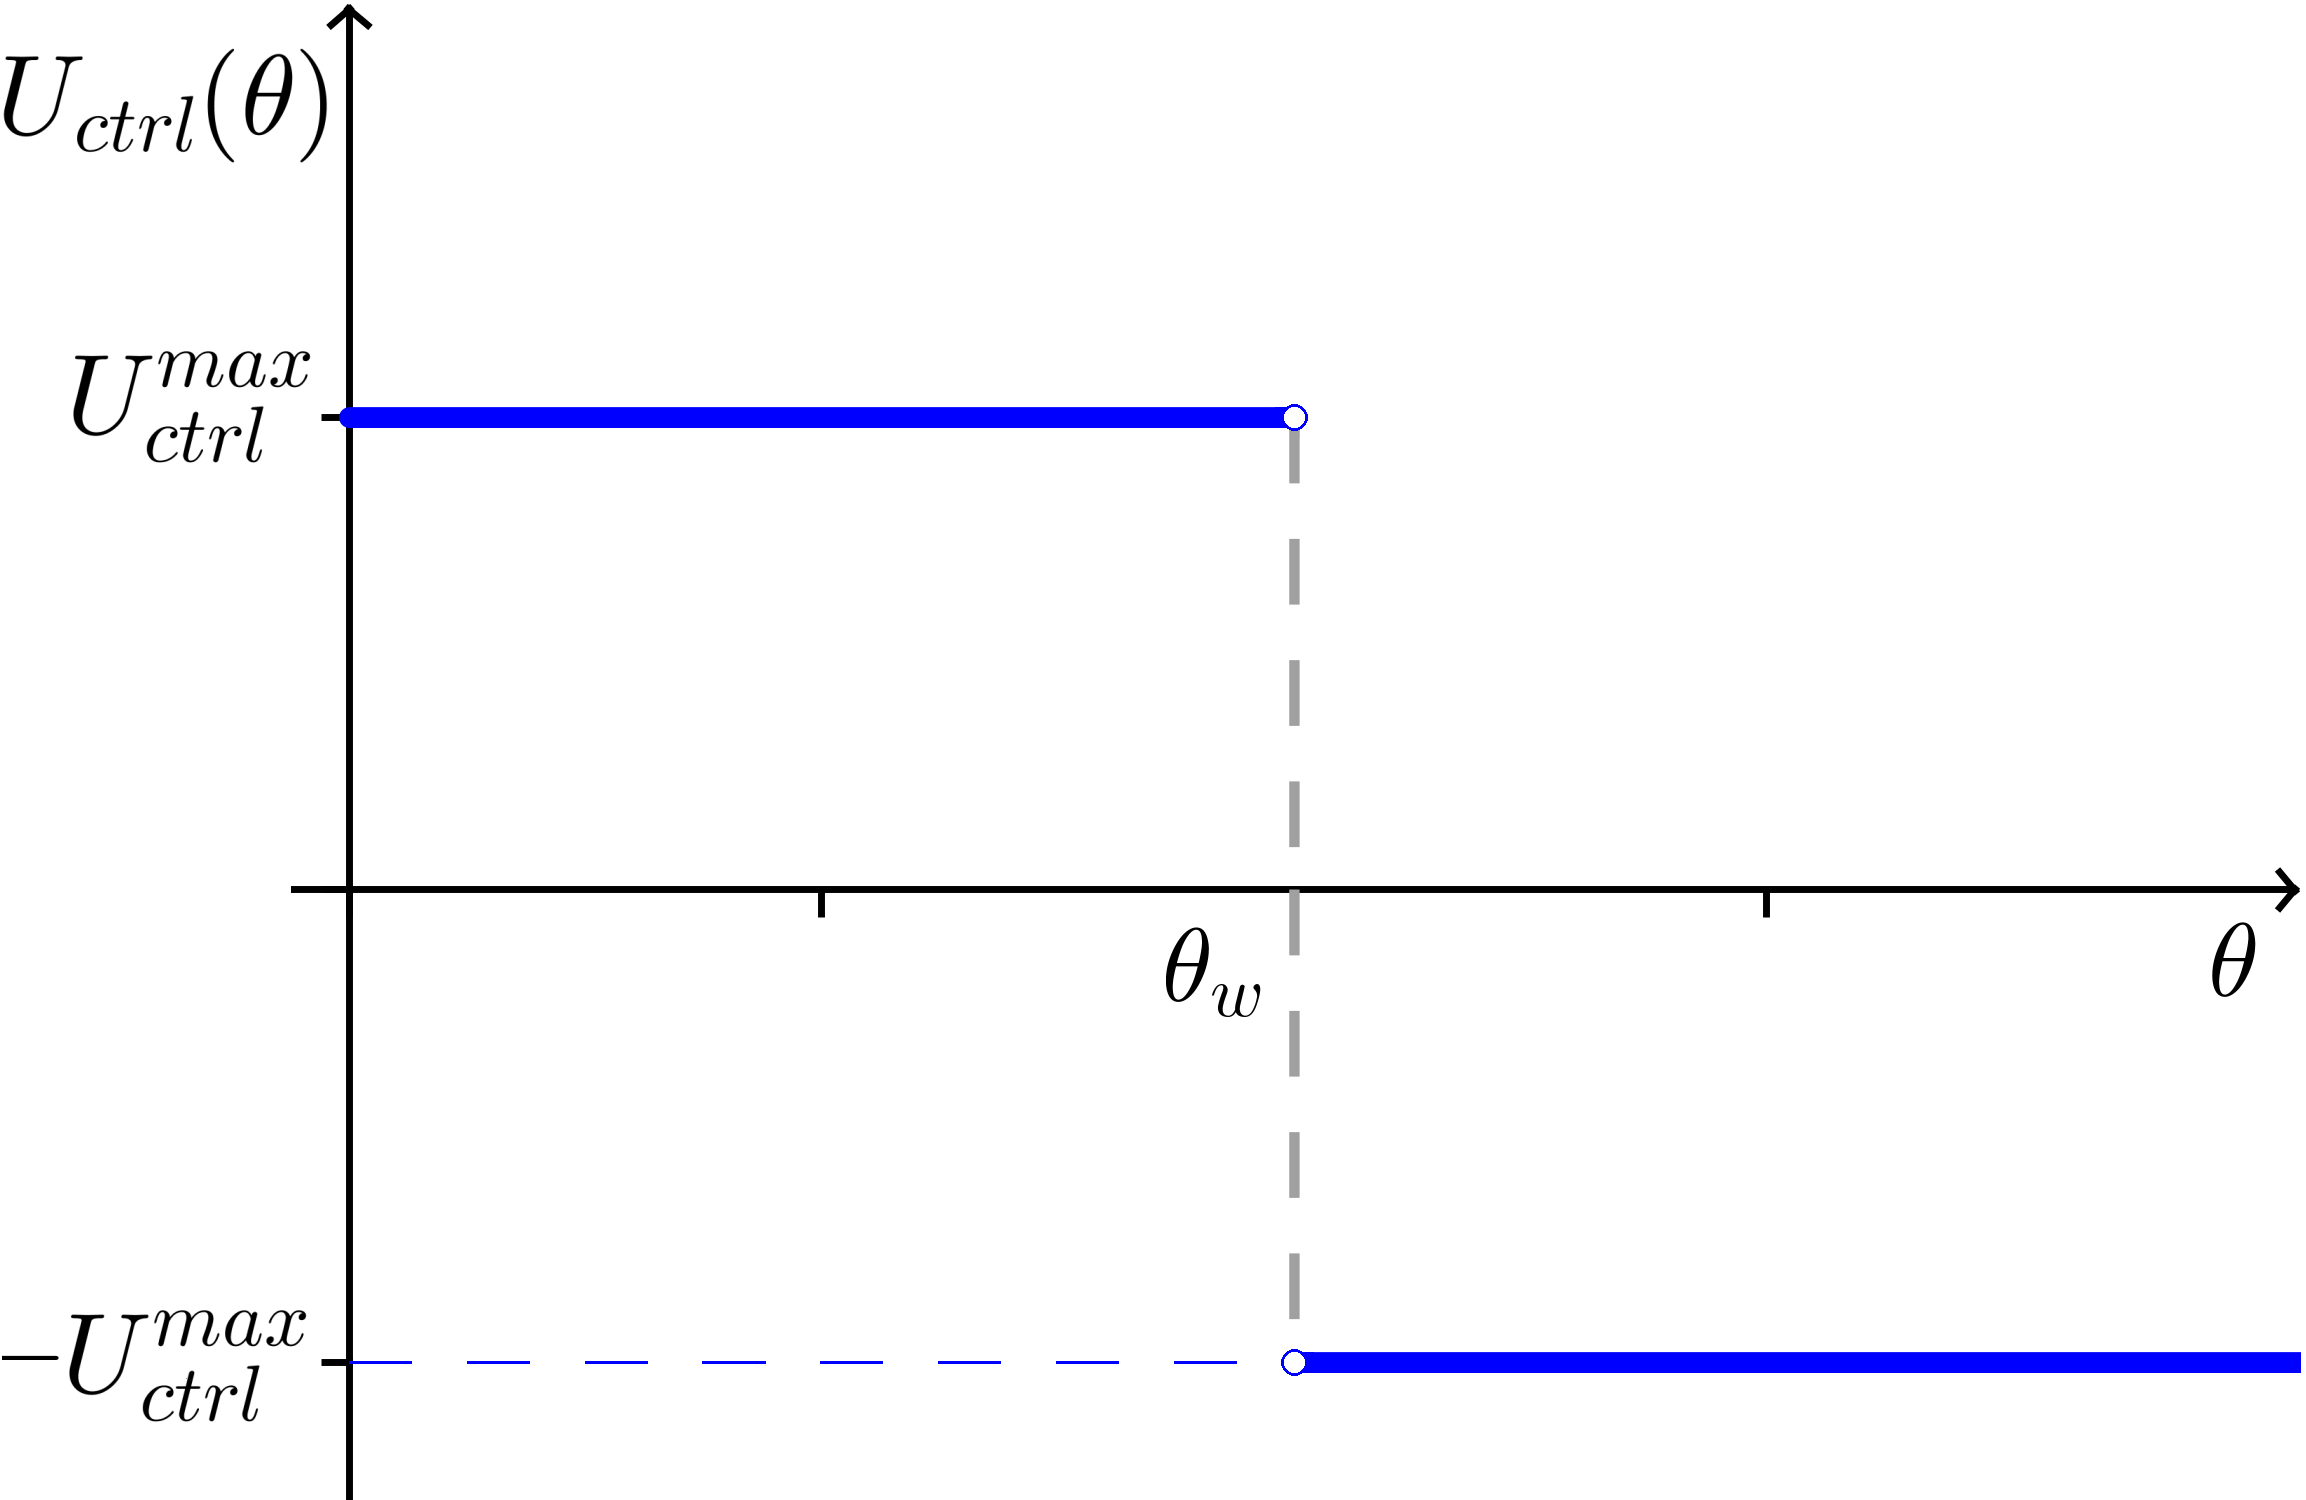
\includegraphics[scale=1]{2_graph.png} }
	\caption{Вид графика после введения в стратегию тормозящего воздействия.}
	\label{2_graph}
\end{figure}

Надо сказать, что данный алгоритм действительно может решить обозначенную проблему, но только в том случае, если силы трения, действующие на механизмы мотора, будут значительны, по сравнению с тем силовым воздействием, которое он испытывает от подачи на него максимального напряжения.
При данном условии вал мотора, совершая затухающее колебательное движение вокруг необходимого положения, в конце концов остановится в нем.
В~другой же ситуации, когда силы трения являются небольшими, описанная стратегия окажется никуда негодной, потому что или процесс торможения вала начнет занимать внушительный промежуток времени, или, в крайнем случае, упомянутые колебания перестанут быть затухающими.

Единственное решение обозначенной проблемы видится в том, чтобы снизить разгоняющее мотор управляющее напряжение, ведь именно при таком раскладе оно будет в меньшей степени <<мешать>> тормозящему действию сил сопротивления.
Однако просто ограничить, например вполовину, абсолютное значение подаваемого напряжения (рис.~\ref{3_graph}) нам никак нельзя. 
Хотя это действие и может вызвать желаемый результат, помимо этого оно в худшую сторону скажется на таком важном для технических приспособлений параметре, как \textit{быcтродействие}.

\begin{figure}[h]
	\noindent\centering{ 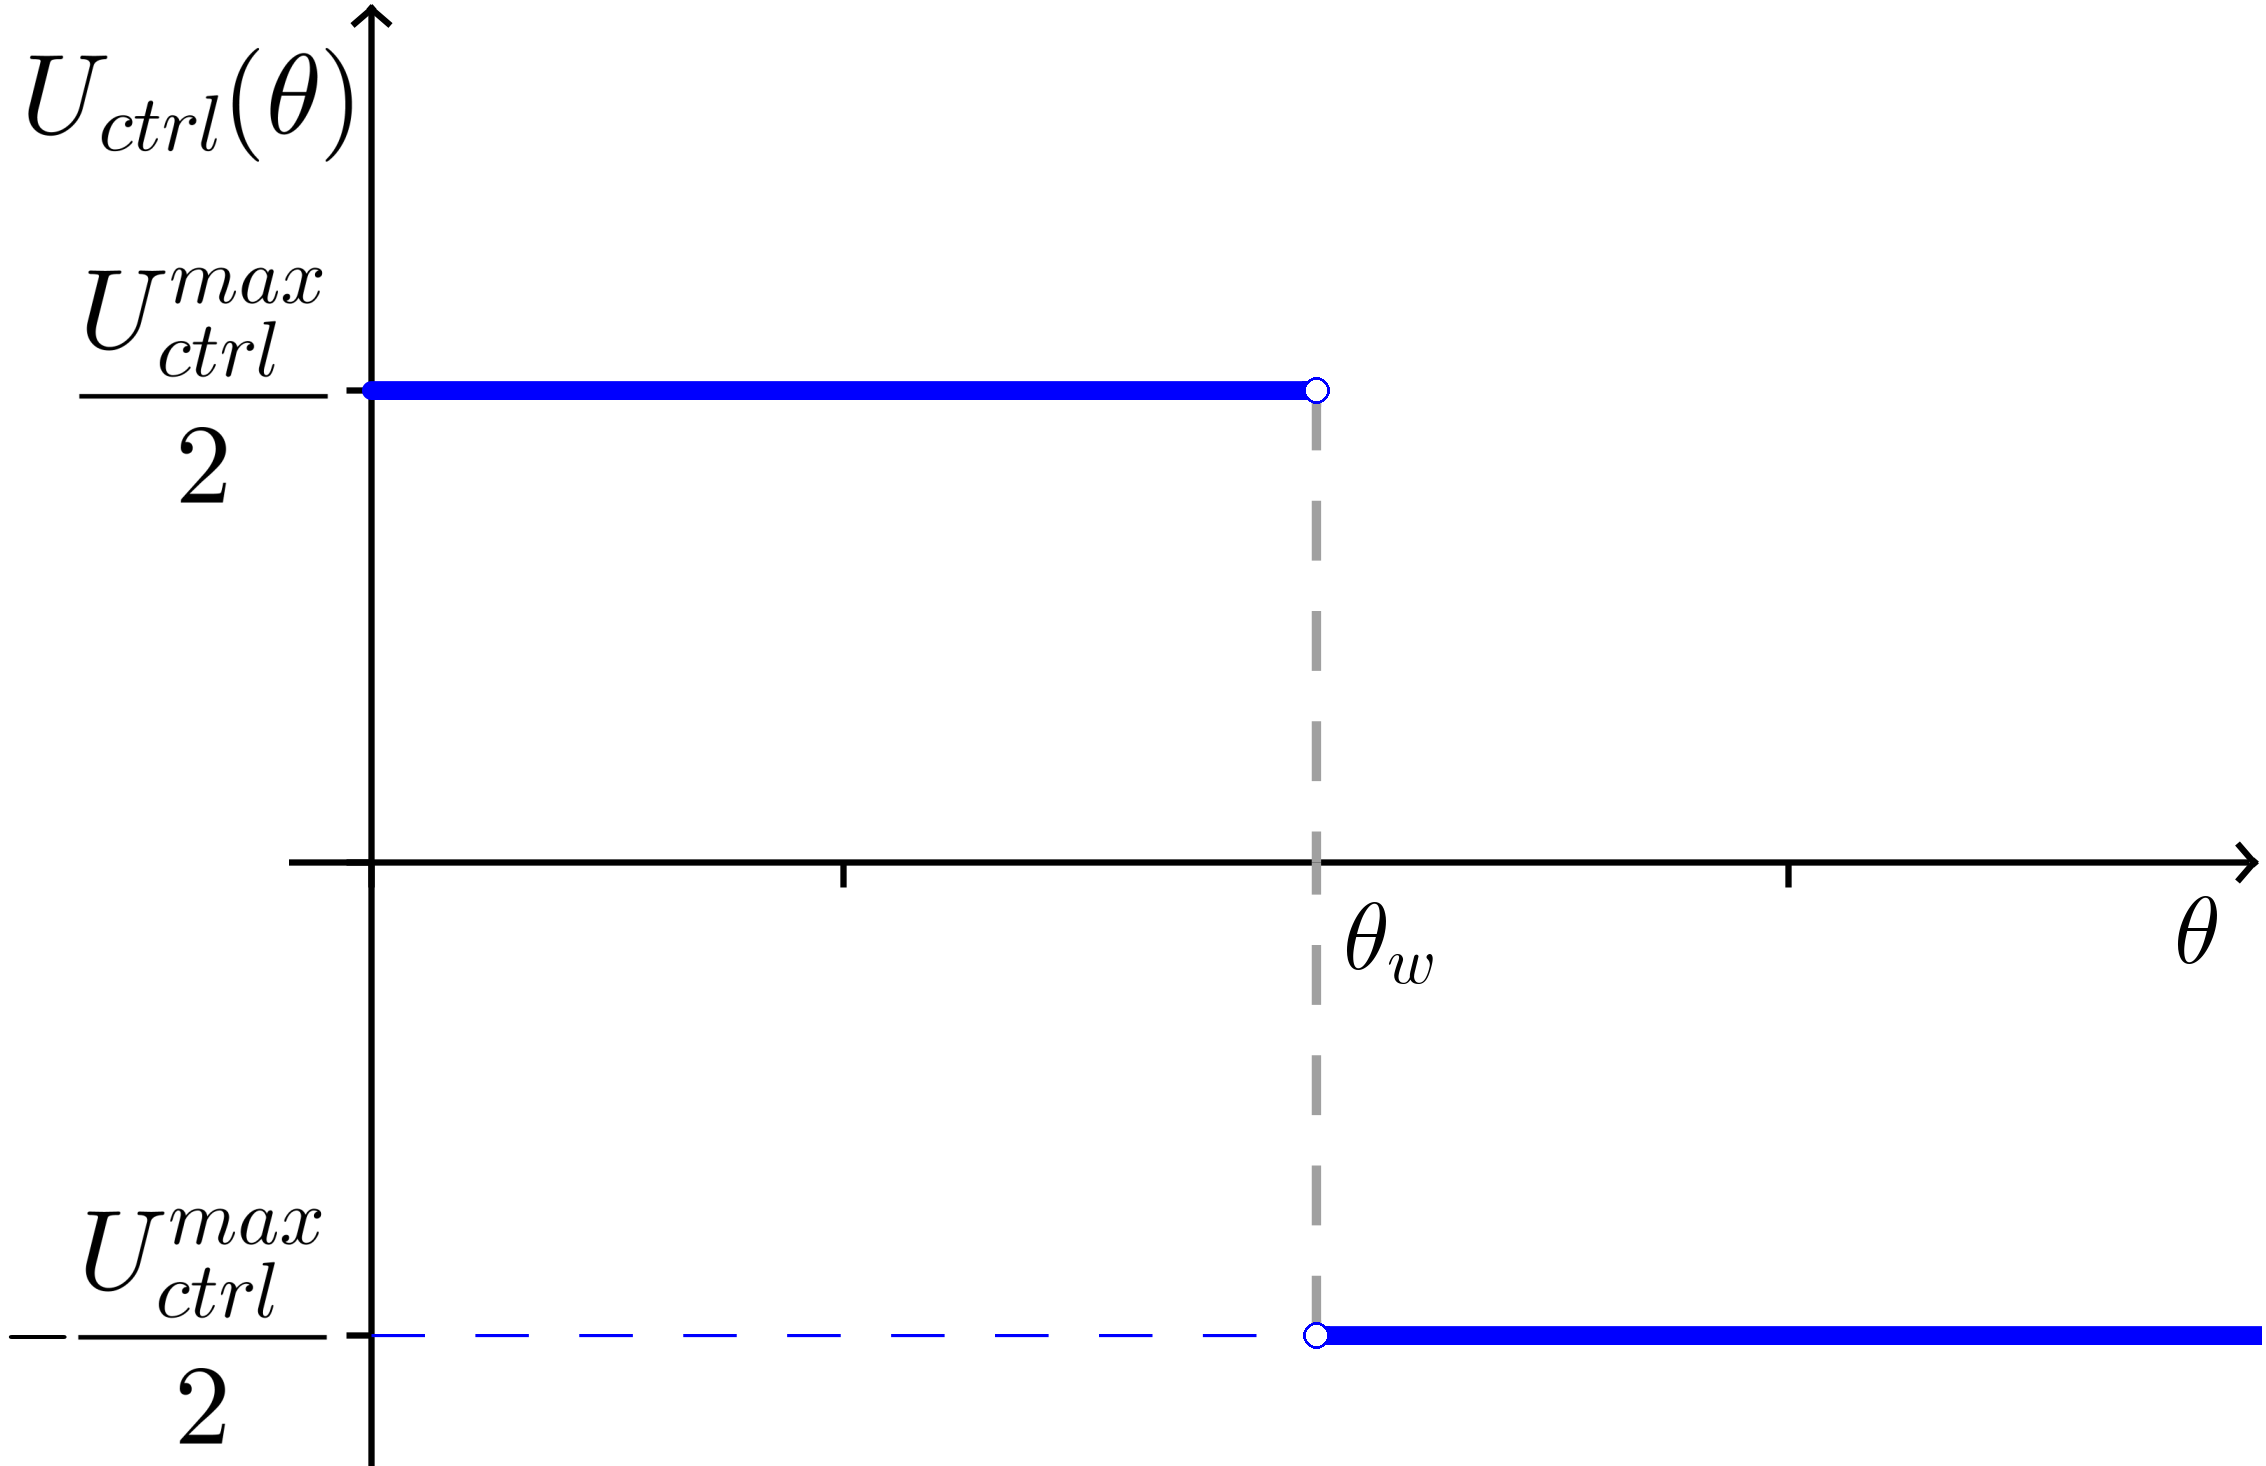
\includegraphics[scale=1]{3_graph.png} }
	\caption{График еще одной неподходящей стратегии.}
	\label{3_graph}
\end{figure}

Учитывая упомянутый аспект, способствовать уменьшению возвращающих вал в необходимое положение сил все-таки можно.
Для этого достаточно снижать управляющее напряжение с некоторого <<расстояния>> от заданного угла.
Пример соответствующей данному подходу зависимости $U_{ctrl}(\theta)$ можно видеть на рис.~\ref{4_graph}, а выражение для нее~--- ниже по тексту:
\begin{equation}\label{for_stairs}
	U_{ctrl}(\theta) =
	\left\{
	\begin{aligned}
		\!U_{ctrl}^{max}\!&, &&\theta \leqslant \frac{\theta_w}{2};\\
		\!\frac{\!U_{ctrl}^{max}}{2}&, &&\frac{\theta_w}{2} < \theta < \theta_w;\\ 
		\!0&, &&\theta = \theta_w;\\
		\!-\frac{\!U_{ctrl}^{max}}{2}&, &&\theta_w < \theta < \frac{3\theta_w}{2};\\	
		\!-U_{ctrl}^{max}\!&, &&\theta \geqslant \frac{3\theta_w}{2};	
	\end{aligned}
	\right.
\end{equation}

Это нововведение, конечно, внесет в используемую стратегию определенный положительный эффект.
Теперь нужное поведение вала будет обеспечено в том числе и в моторах, в которых действуют несколько меньшие силы сопротивления, но та часть механизмов, которая характеризуется еще более незначительными силами сопротивления, откажется должным образом работать и в этом случае.

\begin{figure}[h]
	\noindent\centering{ 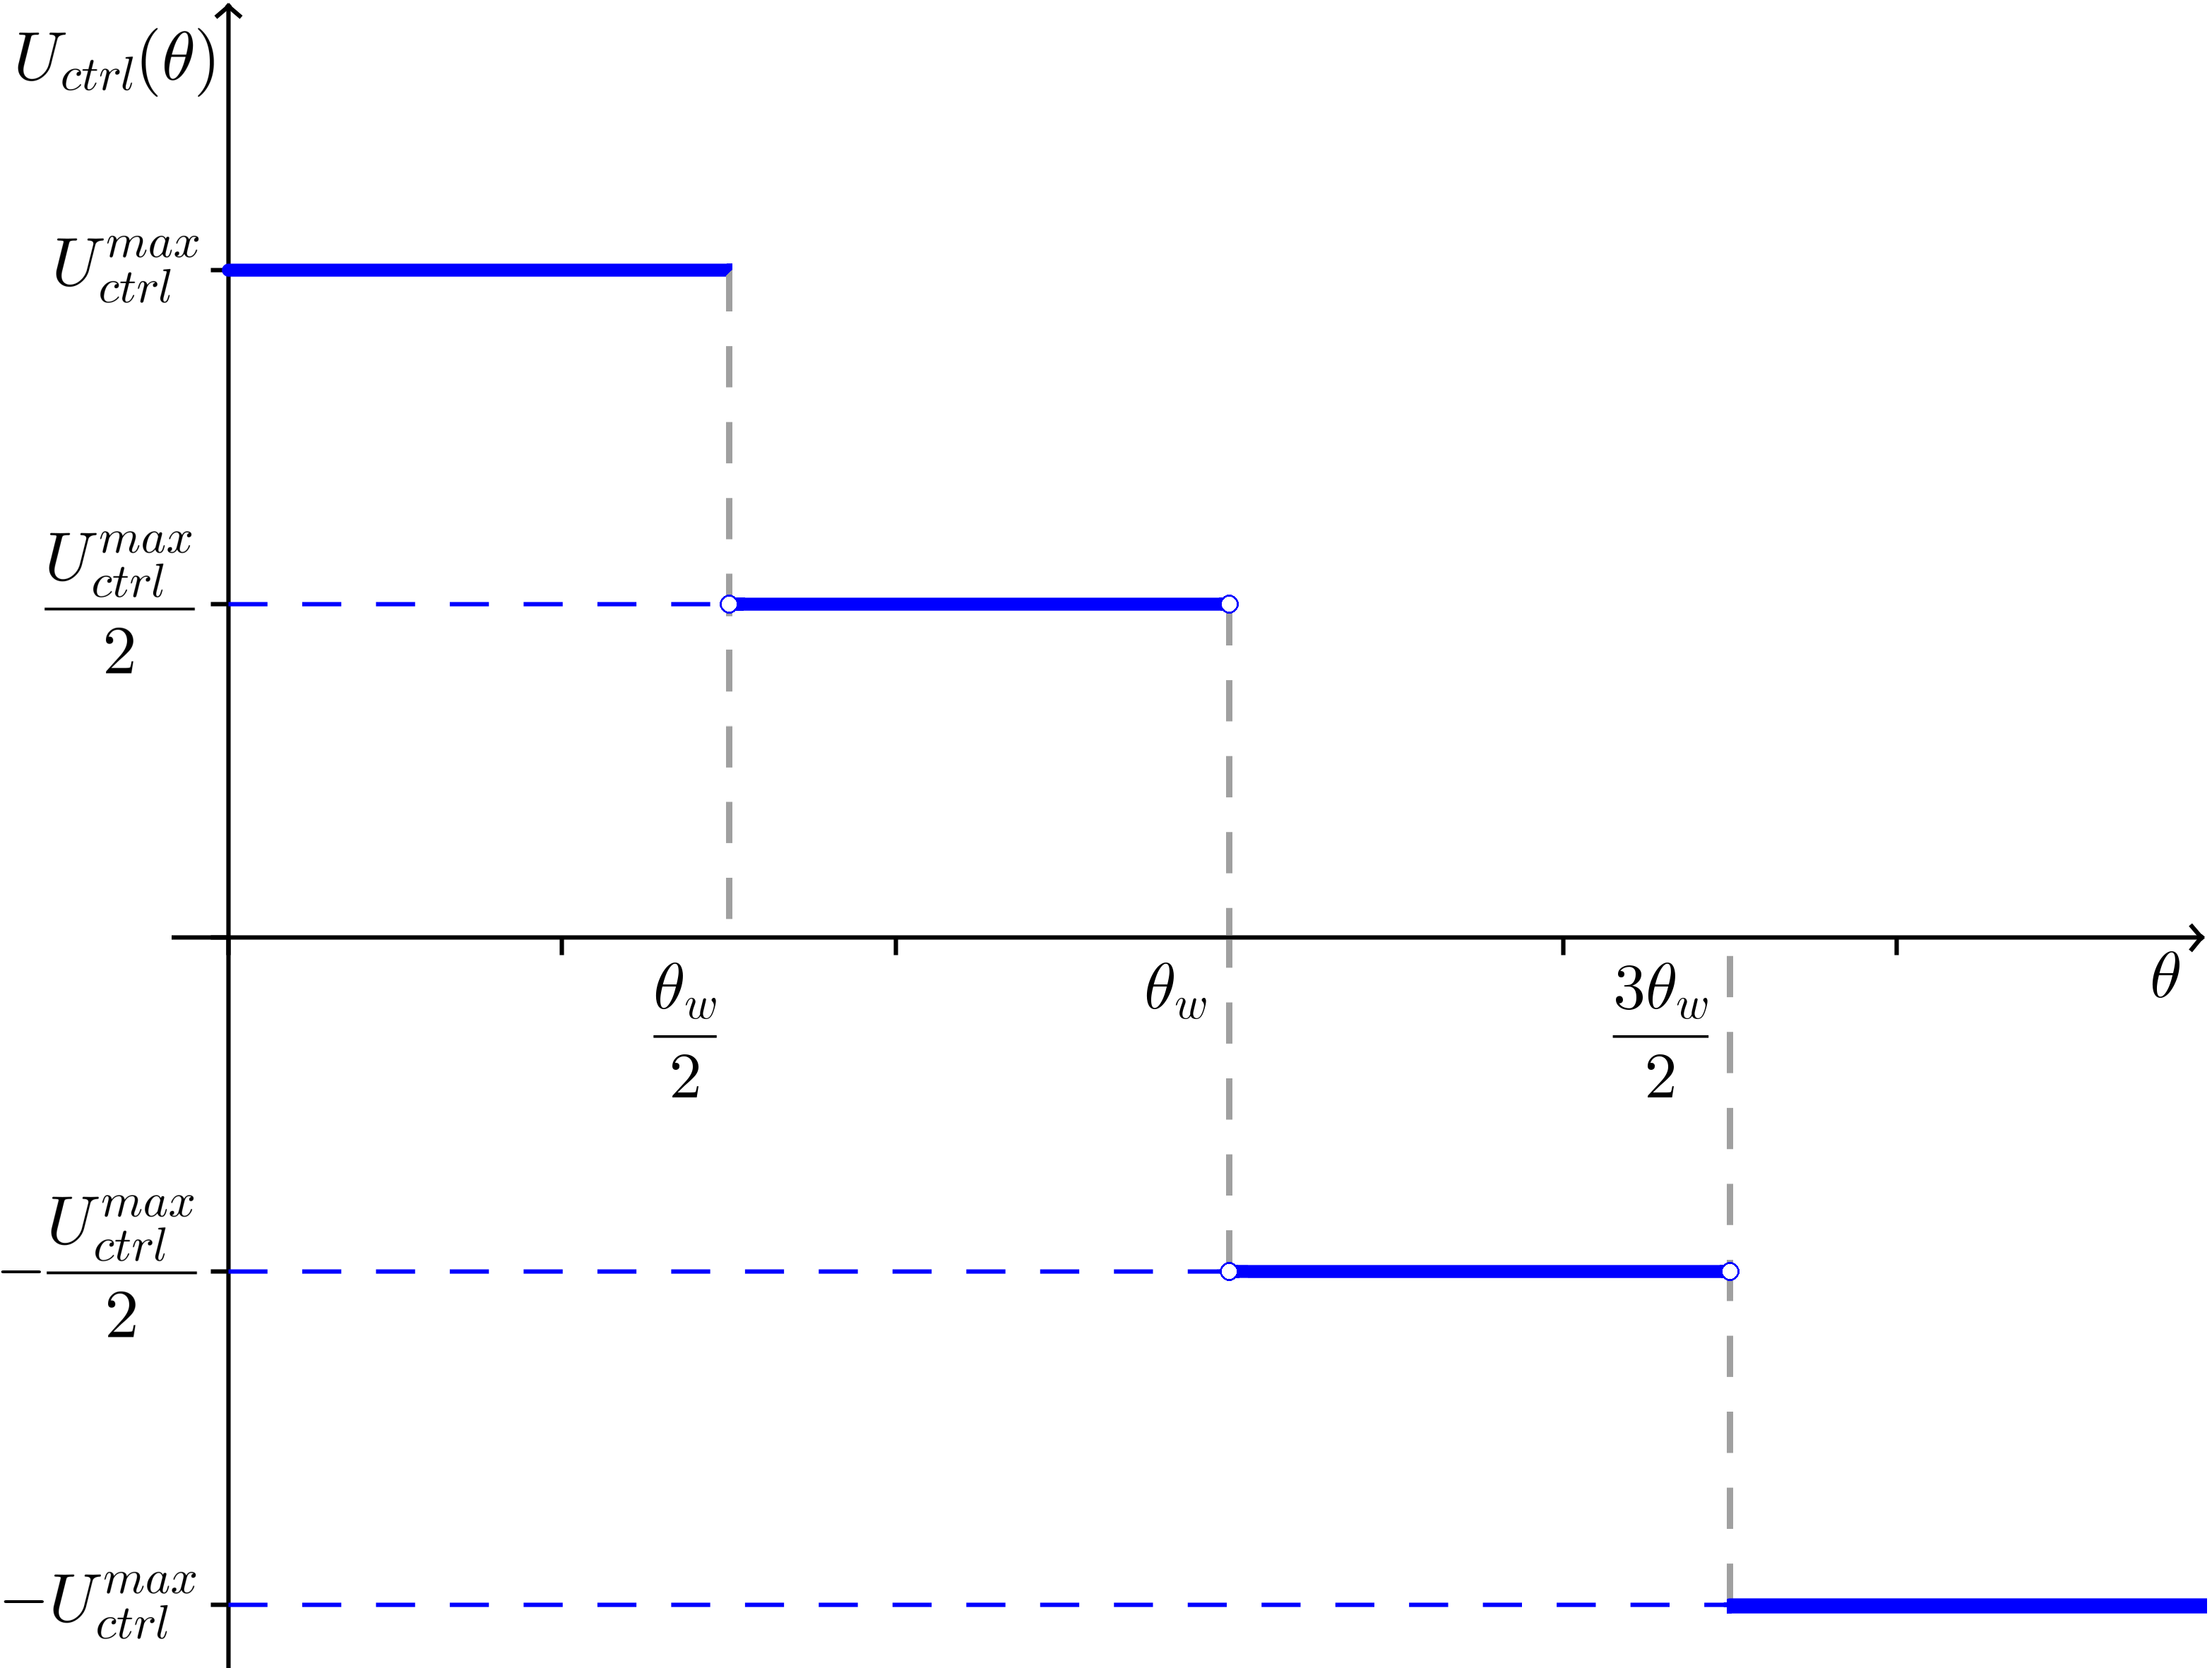
\includegraphics[scale=1]{4_graph.png} }
	\caption{Ступенчатая подача напряжения.}
	\label{4_graph}
\end{figure}

В~данной ситуации не остается ничего более подходящего, чем еще существеннее снижать управляющее напряжение, однако при этом в зависимости от выбранного пути возникнет сразу две проблемы.

Первая из них появится, если мы захотим добиться необходимого эффекта, изменяя продолжительность <<cтупенек>> и напряжение на некоторых из них (рис.~\ref{5_graph}).
Заключается она в том, что при данных условиях мы потеряем \textit{универсальность} искомого алгоритма, то есть он будет работоспособен только по отношению к рассматриваемому мотору.

\begin{figure}[h]
	\noindent\centering{ 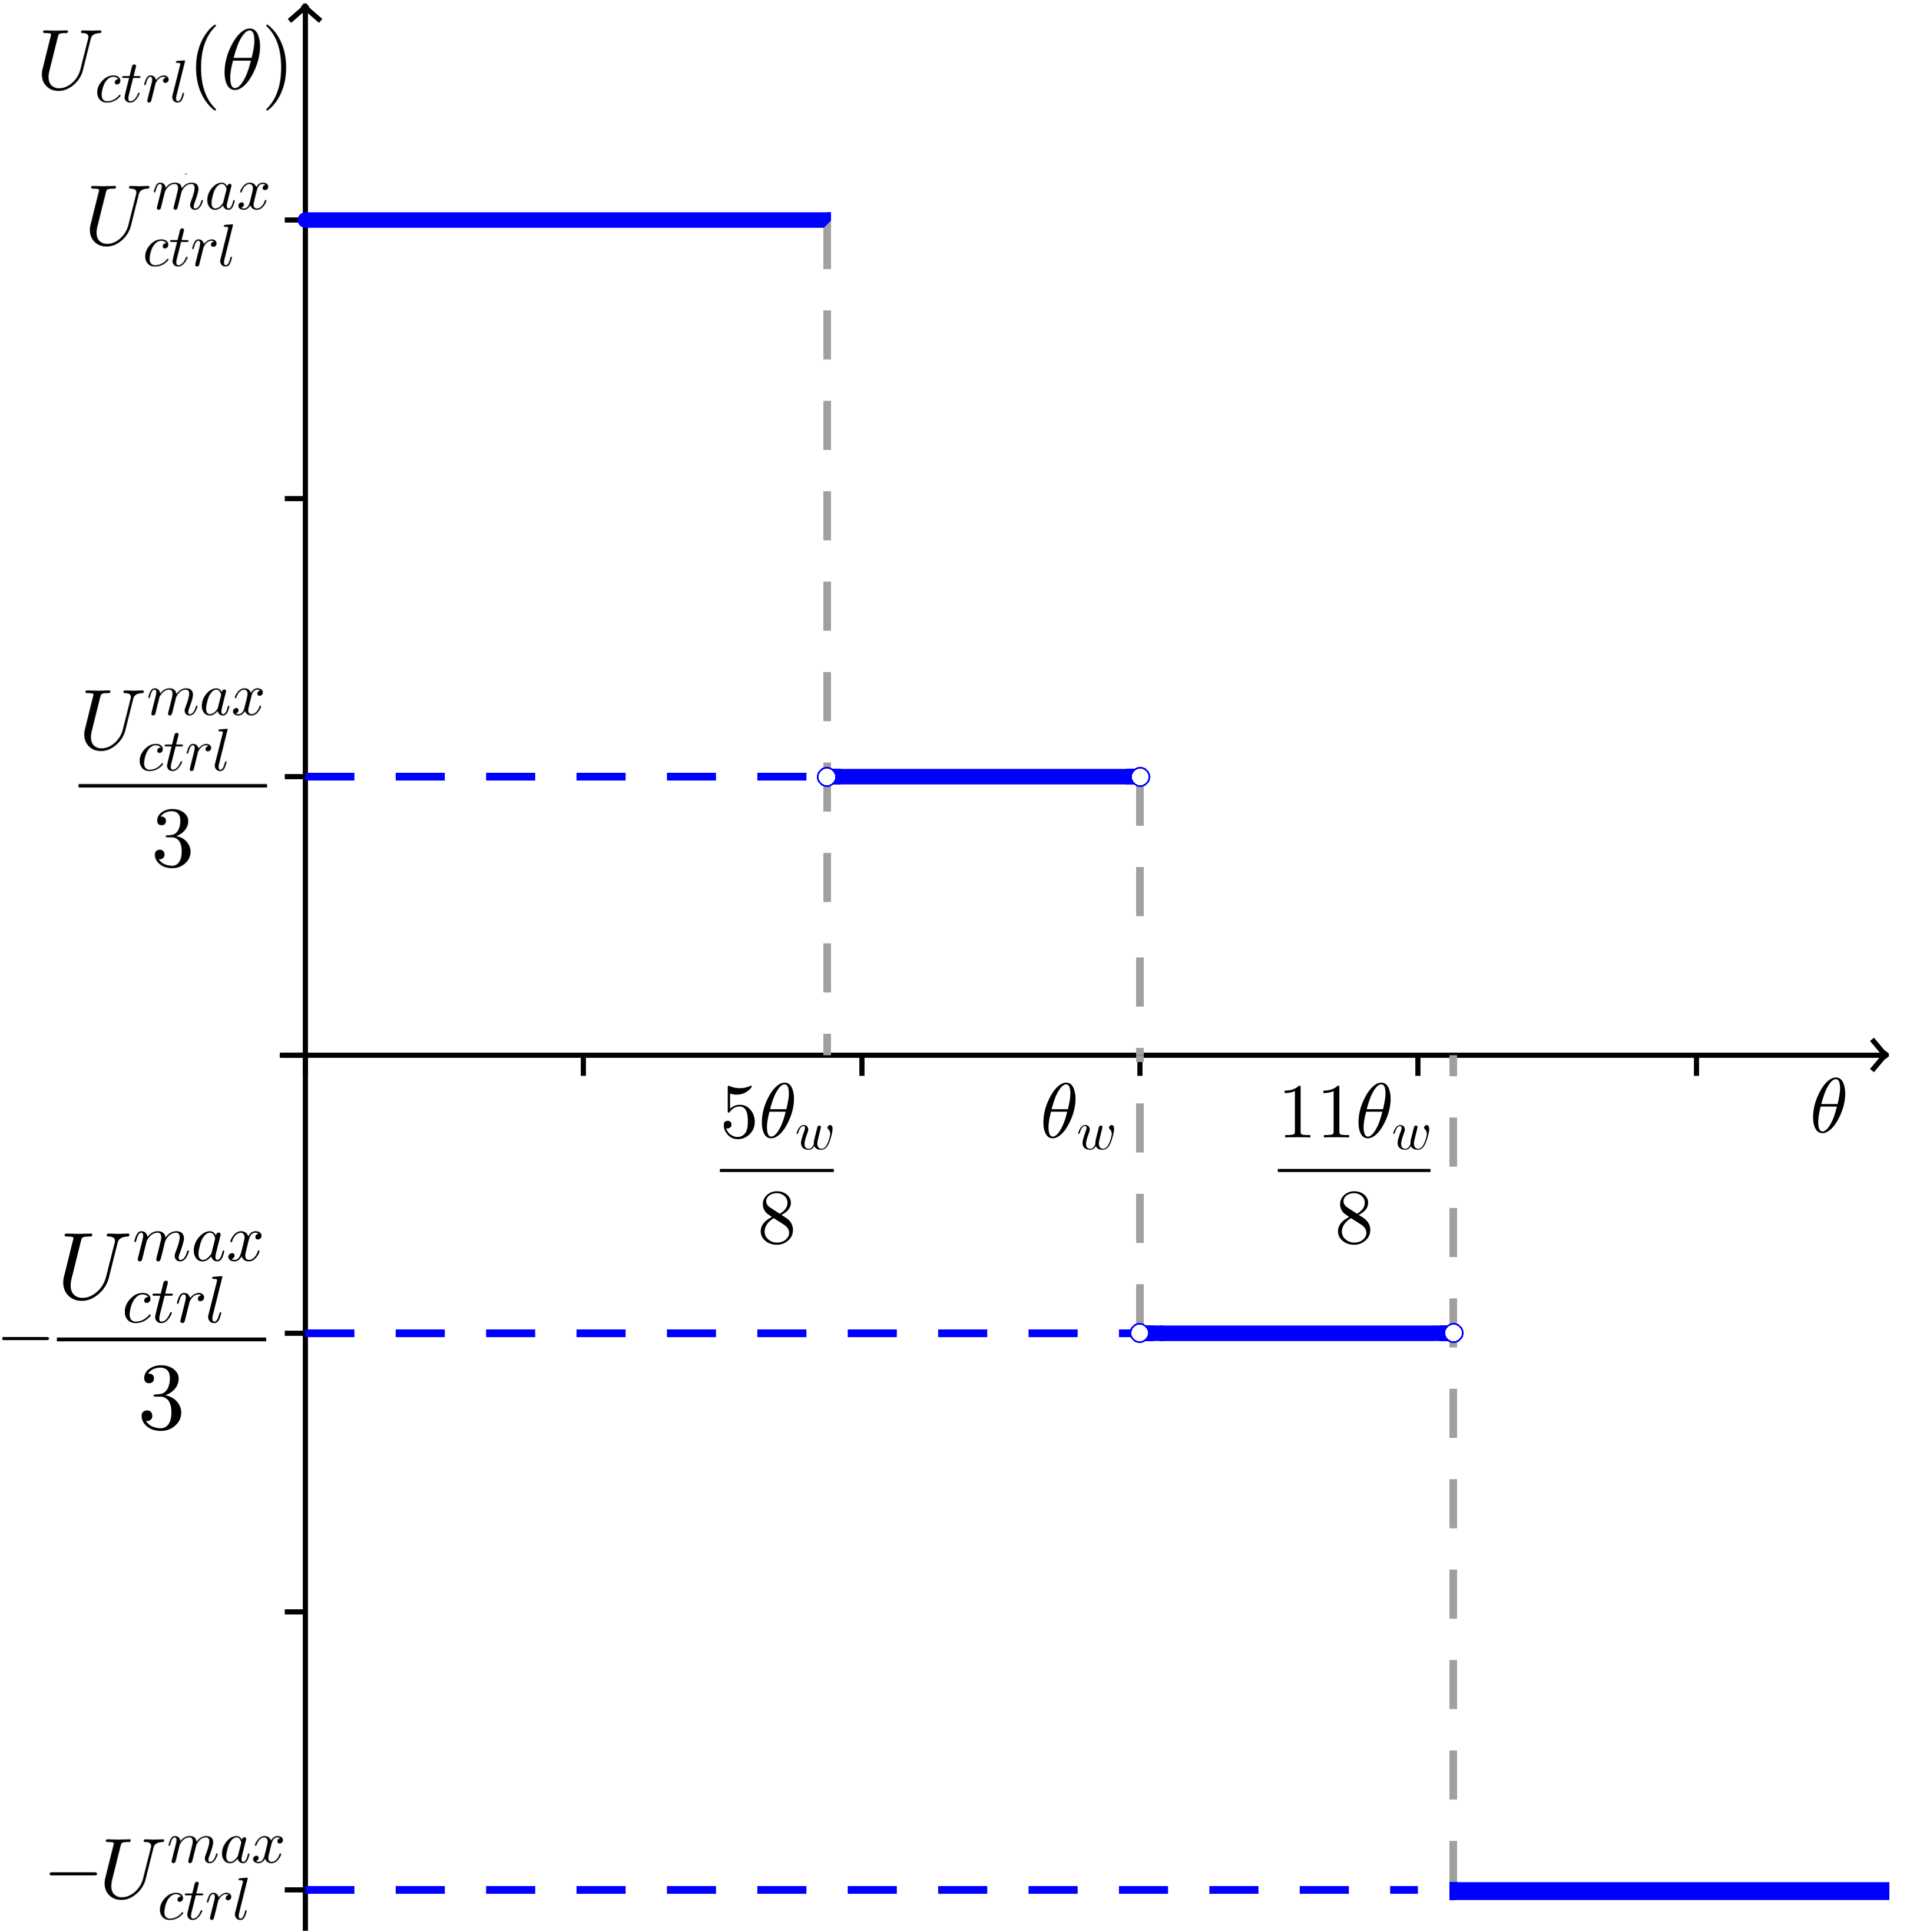
\includegraphics[scale=0.7]{5_graph.png} }
	\caption{Пример изменения параметров <<ступенек>>.}
	\label{5_graph}
\end{figure}

Вторая проблема в полной мере возникнет тогда, когда мы захотим увеличить количество <<ступенек>> (рис.~\ref{6_graph}).
В~этом случае будет усложняться аналитическое выражение зависимости $U_{ctrl}(\theta)$, что, в свою очередь, негативно скажется на простоте технической реализации управляющей стратегии. Несмотря на это, мы пойдем именно этим путем, потому что наша цель~--- выявление \underline{универсального} алгоритма, который можно будет использовать в дальнейшем.

\begin{figure}[h]
	\noindent\centering{ 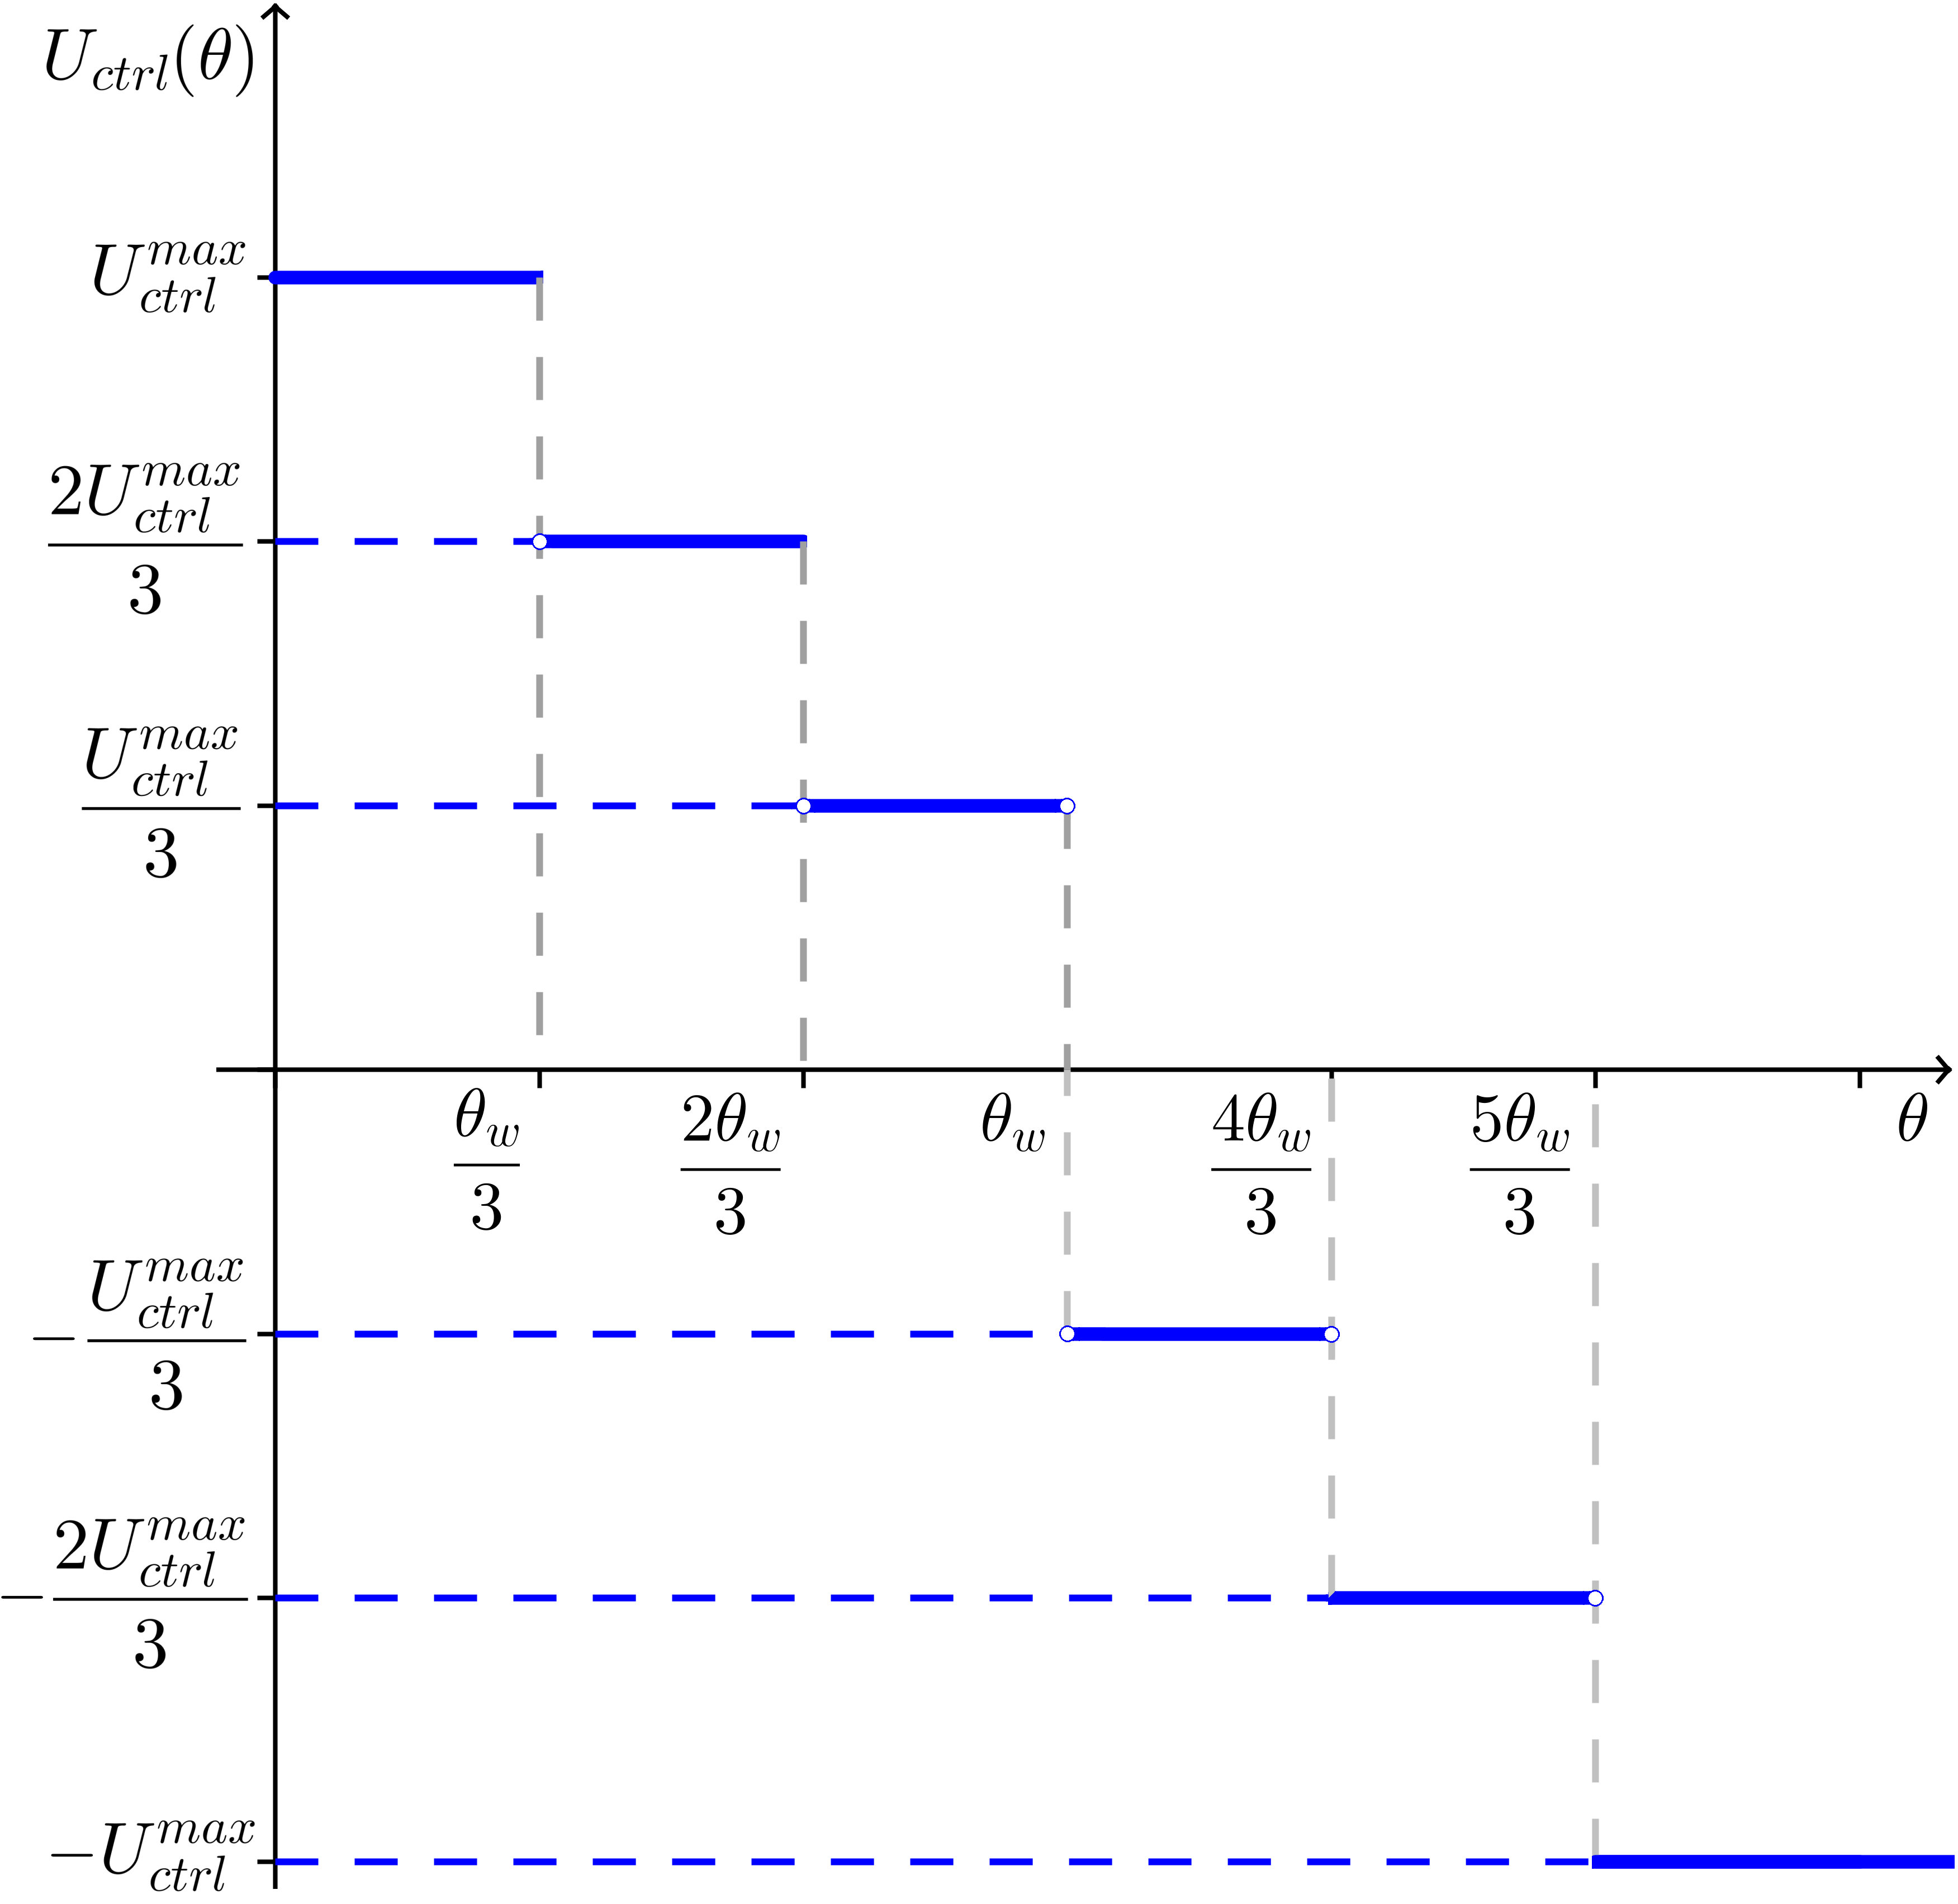
\includegraphics[scale=0.7]{6_graph.png} }
	\caption{Увеличение числа <<ступенек>>.}
	\label{6_graph}
\end{figure}

Поскольку пример аналитической записи зависимости $U_{ctrl}(\theta)$, имеющей <<ступеньки>>, нам дает выше рассмотренный образец (см. рис.~\ref{4_graph} и формулу~\eqref{for_stairs}), не будем заострять на этом внимание и рассмотрим, используя одни только графики, что будет происходить, если увеличивать количество первых.

Очевидно (см. серию рис.~\ref{upstairs}), что при относительно небольшом возрастании числа <<ступенек>> ничего качественно нового в процессе наблюдаться не будет, а все происходящие изменения будут вызывать только еще большее усложнение имеющегося математического уравнения для управляющего воздействия.
Однако, по мере приближения количества <<ступенек>> к бесконечности график зависимости $U_{ctrl}(\theta)$ все отчетливее будет становиться похожим на график обычной линейной функции.
Это очень хороший результат.
Принимая для управляющего воздействия именно такой закон изменения, мы, не теряя основного предназначения всех выше приведенных трансформаций\lefteqn,\footnote{Имеется в виду уменьшение разгоняющих сил, действующих на вал вблизи заданного положения.} в то же самое время получим легкое для технической реализации выражение, описывающее характер подаваемого напряжения:
\begin{equation}\label{p-controller}
	U_{ctrl}(\theta) = k_\textit{п}(\theta_w - \theta),
\end{equation}
где $k_\textit{п}$~--- некоторый коэффициент пропорциональности ($k_\textit{п} = const$).

\begin{figure}[h!]
	\begin{minipage}[h]{0.47\linewidth}
		\center{ 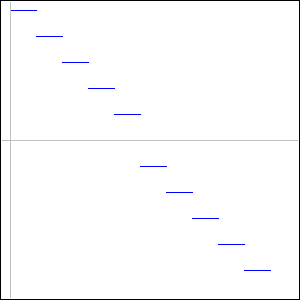
\includegraphics[scale=1]{few.png} \\ a)} 
	\end{minipage}
	\hfill
	\begin{minipage}[h]{0.47\linewidth}
		\center{ 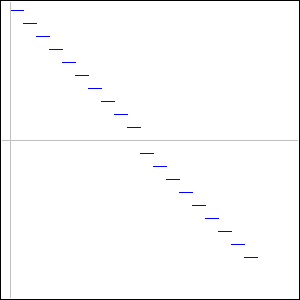
\includegraphics[scale=1]{more.png} \\ б)}
	\end{minipage}
	\vfill
	\begin{minipage}[h]{0.47\linewidth}
		\center{ 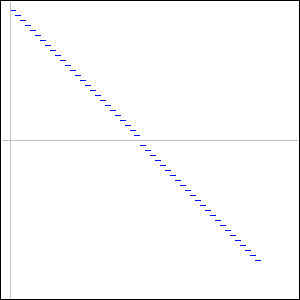
\includegraphics[scale=1]{many.png} \\ в)} 
	\end{minipage}
	\hfill
	\begin{minipage}[h]{0.47\linewidth}
		\center{ 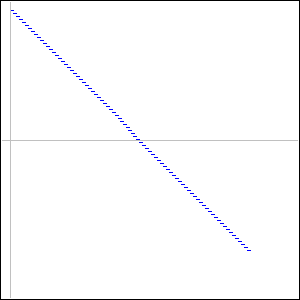
\includegraphics[scale=1]{infinity.png} \\ г)}
	\end{minipage}
	\caption{Процесс еще большего увеличения числа <<ступенек>>.}
	\label{upstairs}
\end{figure}

Теперь остается добавить, что полученная стратегия и есть искомый П-регулятор.
C~его помощью мы действительно можем добиться нужного поведения вала любого мотора, да и не только.
Единственное, что при этом останется сделать~--- это подобрать подходящее значение постоянной $k_\textit{п}$\footnote{Выше, в формуле~\eqref{p-controller}, мы не написали на его месте напрашивающегося числового значения $U_{ctrl}^{max}\!/\theta_w$ по той причине, что значение $k_\textit{п}$, не нарушая работоспособности управляющей стратегии, может быть и другим.} или рассчитать его на основе конкретных методов.
Надо сказать, что бывают случаи, когда значения этого коэффициента могут лежать в очень широком диапазоне.
Примеры как раз таких задач предстоит разобрать в практической части данной лабораторной работы.

В~завершение подведем итог и заключим, что под П-регулятором понимается такая стратегия управления, при которой в качестве управляющего воздействия в систему подается сигнал, чье значение в каждый момент времени рассчитывается, как произведение некоторого постоянного числового коэффициента на разность текущего значения интересующего нас выходного сигнала и желаемого его значения.
Математическая запись характера управляющего воздействия при этом выглядит следующим образом:
\begin{equation}\label{main_p-contoller}
	u_{c} = k(x_i^*-x_i),
\end{equation}
где $u_c$~--- управляющий сигнал, $k$~--- коэффициент пропорциональности, $x_i$~--- текущее значение рассматриваемого\footnote{Это слово добавлено потому, что выходных сигналов может быть несколько, однако не обязательно, что при этом рассматриваться будут все.
Например, в нашей задаче мы вообще не интересуемся поведением электродинамических характеристик двигателя, лежащего в основе мотора, а работаем только с угловой координатой выходного вала последнего.} выходного сигнала, $x_i^*$~--- желаемое значение последнего.

\paragraph*{Проверка результата}$\phantom{-}$\\
\hspace*{\parindent}Для того чтобы подтвердить работоспособность найденного алгоритма до начала работы над каким-либо устройством, воспользуемся схемой моделирования рассматриваемого процесса.
К~решению дифференциальных уравнений в этот раз прибегать не будем.  

Поскольку мы рассматриваем некоторый процесс, происходящий в моторе EV3, то очевидно, что основу его (процесса) схемы моделирования будет составлять схема работы мотора (в прошлой работе мы обвели ее зеленым контуром).
При этом останется только сформировать входящее воздействие согласно уравнению~\eqref{p-controller} и добавить в схему блоки, которые позволят получать на выходе значения зависимости $\theta(t)$.
Итог~--- см.~рис.~\ref{struct_sheme}.

\begin{figure}[h]
	\centering{ 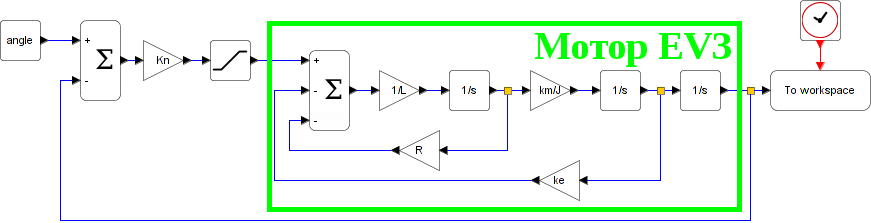
\includegraphics[scale=0.6]{struct_sheme_ev3.png} }
	\caption{Схема моделирования процесса.}
	\label{struct_sheme}
\end{figure}

Несложно догадаться, что в переменной angle хранится значение того угла, на который должен повернуться вал мотора\lefteqn,\footnote{Обратите внимание на то, что используемые в схеме моделирования значения углов выражаются в радианах.} а в Kn~--- значение коэффициента пропорциональности.
Блок с изображением ломаной нужен для следующего.
Вычисленное по формуле~\eqref{p-controller} значение напряжения может оказаться слишком большим для того, чтобы его можно было обеспечить источником питания блока EV3.
В~этом случае логичнее всего заменить полученный результат значением максимального напряжения, на которое рассчитана используемая батарея.
Упомянутый блок как раз реализует эту задачу; одним словом, формула его работы применительно к нашему процессу имеет вид:
\begin{equation}
	\mathrm{OUT} = 
	\left\{
	\begin{aligned}
		\!U_{ctrl}^{max}&, &&\mathrm{IN} > U_{ctrl}^{max}; \\
		\!\mathrm{IN}&, &&\mathrm{IN} \in \left[-U_{ctrl}^{max}; U_{ctrl}^{max}\right]; \\
		\!-U_{ctrl}^{max}&, &&\mathrm{IN} < -U_{ctrl}^{max},
	\end{aligned}
	\right.
\end{equation}
где $\mathrm{IN}$~--- сигнал, который подается на вход данного блока, $\mathrm{OUT}$~--- его выходной сигнал.

\newpage				 
\section{Цель работы}
\hspace*{\parindent}Познакомиться с понятием П-регулятора на примере простейшей задачи управления.
Используя полученные знания, построить заданное робототехническое устройство.

\section{Порядок выполнения работы}
\begin{enumerate}
	\item Опытная проверка работоспособности П-регулятора.
	\begin{enumerate}
		\item Соберите такую же, как в первой работе, конструкцию.
		\item Напишите для нее программу на языке Python, которая бы запускала мотор EV3 на вращение и, используя управляющую стратегию П-регулятора, фиксировала его в положении, соответствующем повороту его выходного вала из начального состояния на $180^\circ$\!\!.
		При этом она должна сформировать такой же, как в первой работе, файл с данными.
		
		Заметьте, что в методе класса \verb|LargeMotor.run_direct(duty_cycle_sp)|, подающем напряжение на мотор, значение аргумента задается в процентах от максимального напряжения, которое может обеспечить в данных условиях аккумулятор.
		По этой причине прежде, чем использовать рассчитанное по формуле~\eqref{p-controller} значение управляющего напряжения, его необходимо представить в упомянутом процентном выражении.
		
		Как уже было сказано в теоретической части методического пособия, полученное из расчетов по формуле~\eqref{p-controller} число может превысить максимальное напряжение, выдаваемое источником питания.
		Следовательно, после того, как в программе рассчитывается значение управляющего воздействия и результат переводится в проценты, необходимо дополнительно проверять не выходит ли полученный результат за границы промежутка  $[-100;100]$.
		В случае неудовлетворительного итога проверки полученное значение необходимо заменять на ближайшее к нему число из указанного промежутка, то есть на $100$ или $-100$. 
		Полезной на этом шаге может оказаться функция \verb|copysign(1, arg)| из встроенного модуля \verb|math|.
		Она возвращает единицу, если ее аргумент положителен или равен нулю, $(-1)$, если он отрицательный.
		\item Запустите программу на выполнение три раза, меняя в каждом из них значение коэффициента пропорциональности, использующегося в П-регуляторе.
		Значения коэффициента подберите опытным путем.
		\item На основе полученных данных постройте в Scilab графики зависимости $\theta(t)$.
		\item Постройте согласно рис.~\ref{struct_sheme} схему моделирования исследуемого процесса в Xcos.
		Промоделировав ее для каждого из трех ранее использованных значений коэффициента пропорциональности, постройте в соответствующих окнах получившиеся графики зависимости $\theta(t)$.
		Пример графиков, которые должны получиться~--- см.~рис.~\ref{example}.
		
		\begin{figure}[h!]
			\centering{ 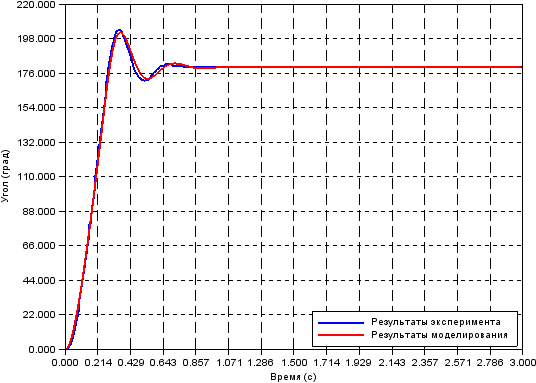
\includegraphics{example.png} }
			\caption{Примеры графиков.}
			\label{example}
		\end{figure}
	\end{enumerate}
	\item Создание робота.
	\begin{enumerate}
		\item Соберите робота-машинку, снабженного(ую) ультразвуковым датчиком~--- дальномером (см.~Приложение~А и рис.~\ref{ultrasonic_sensor}), направленным вдоль линии движения первого(ой).
		Пример требуемого механизма~--- см.~рис.~\ref{robocar}.
		\begin{figure}[h!]
			\begin{minipage}[h]{0.49\linewidth}
				\center{ 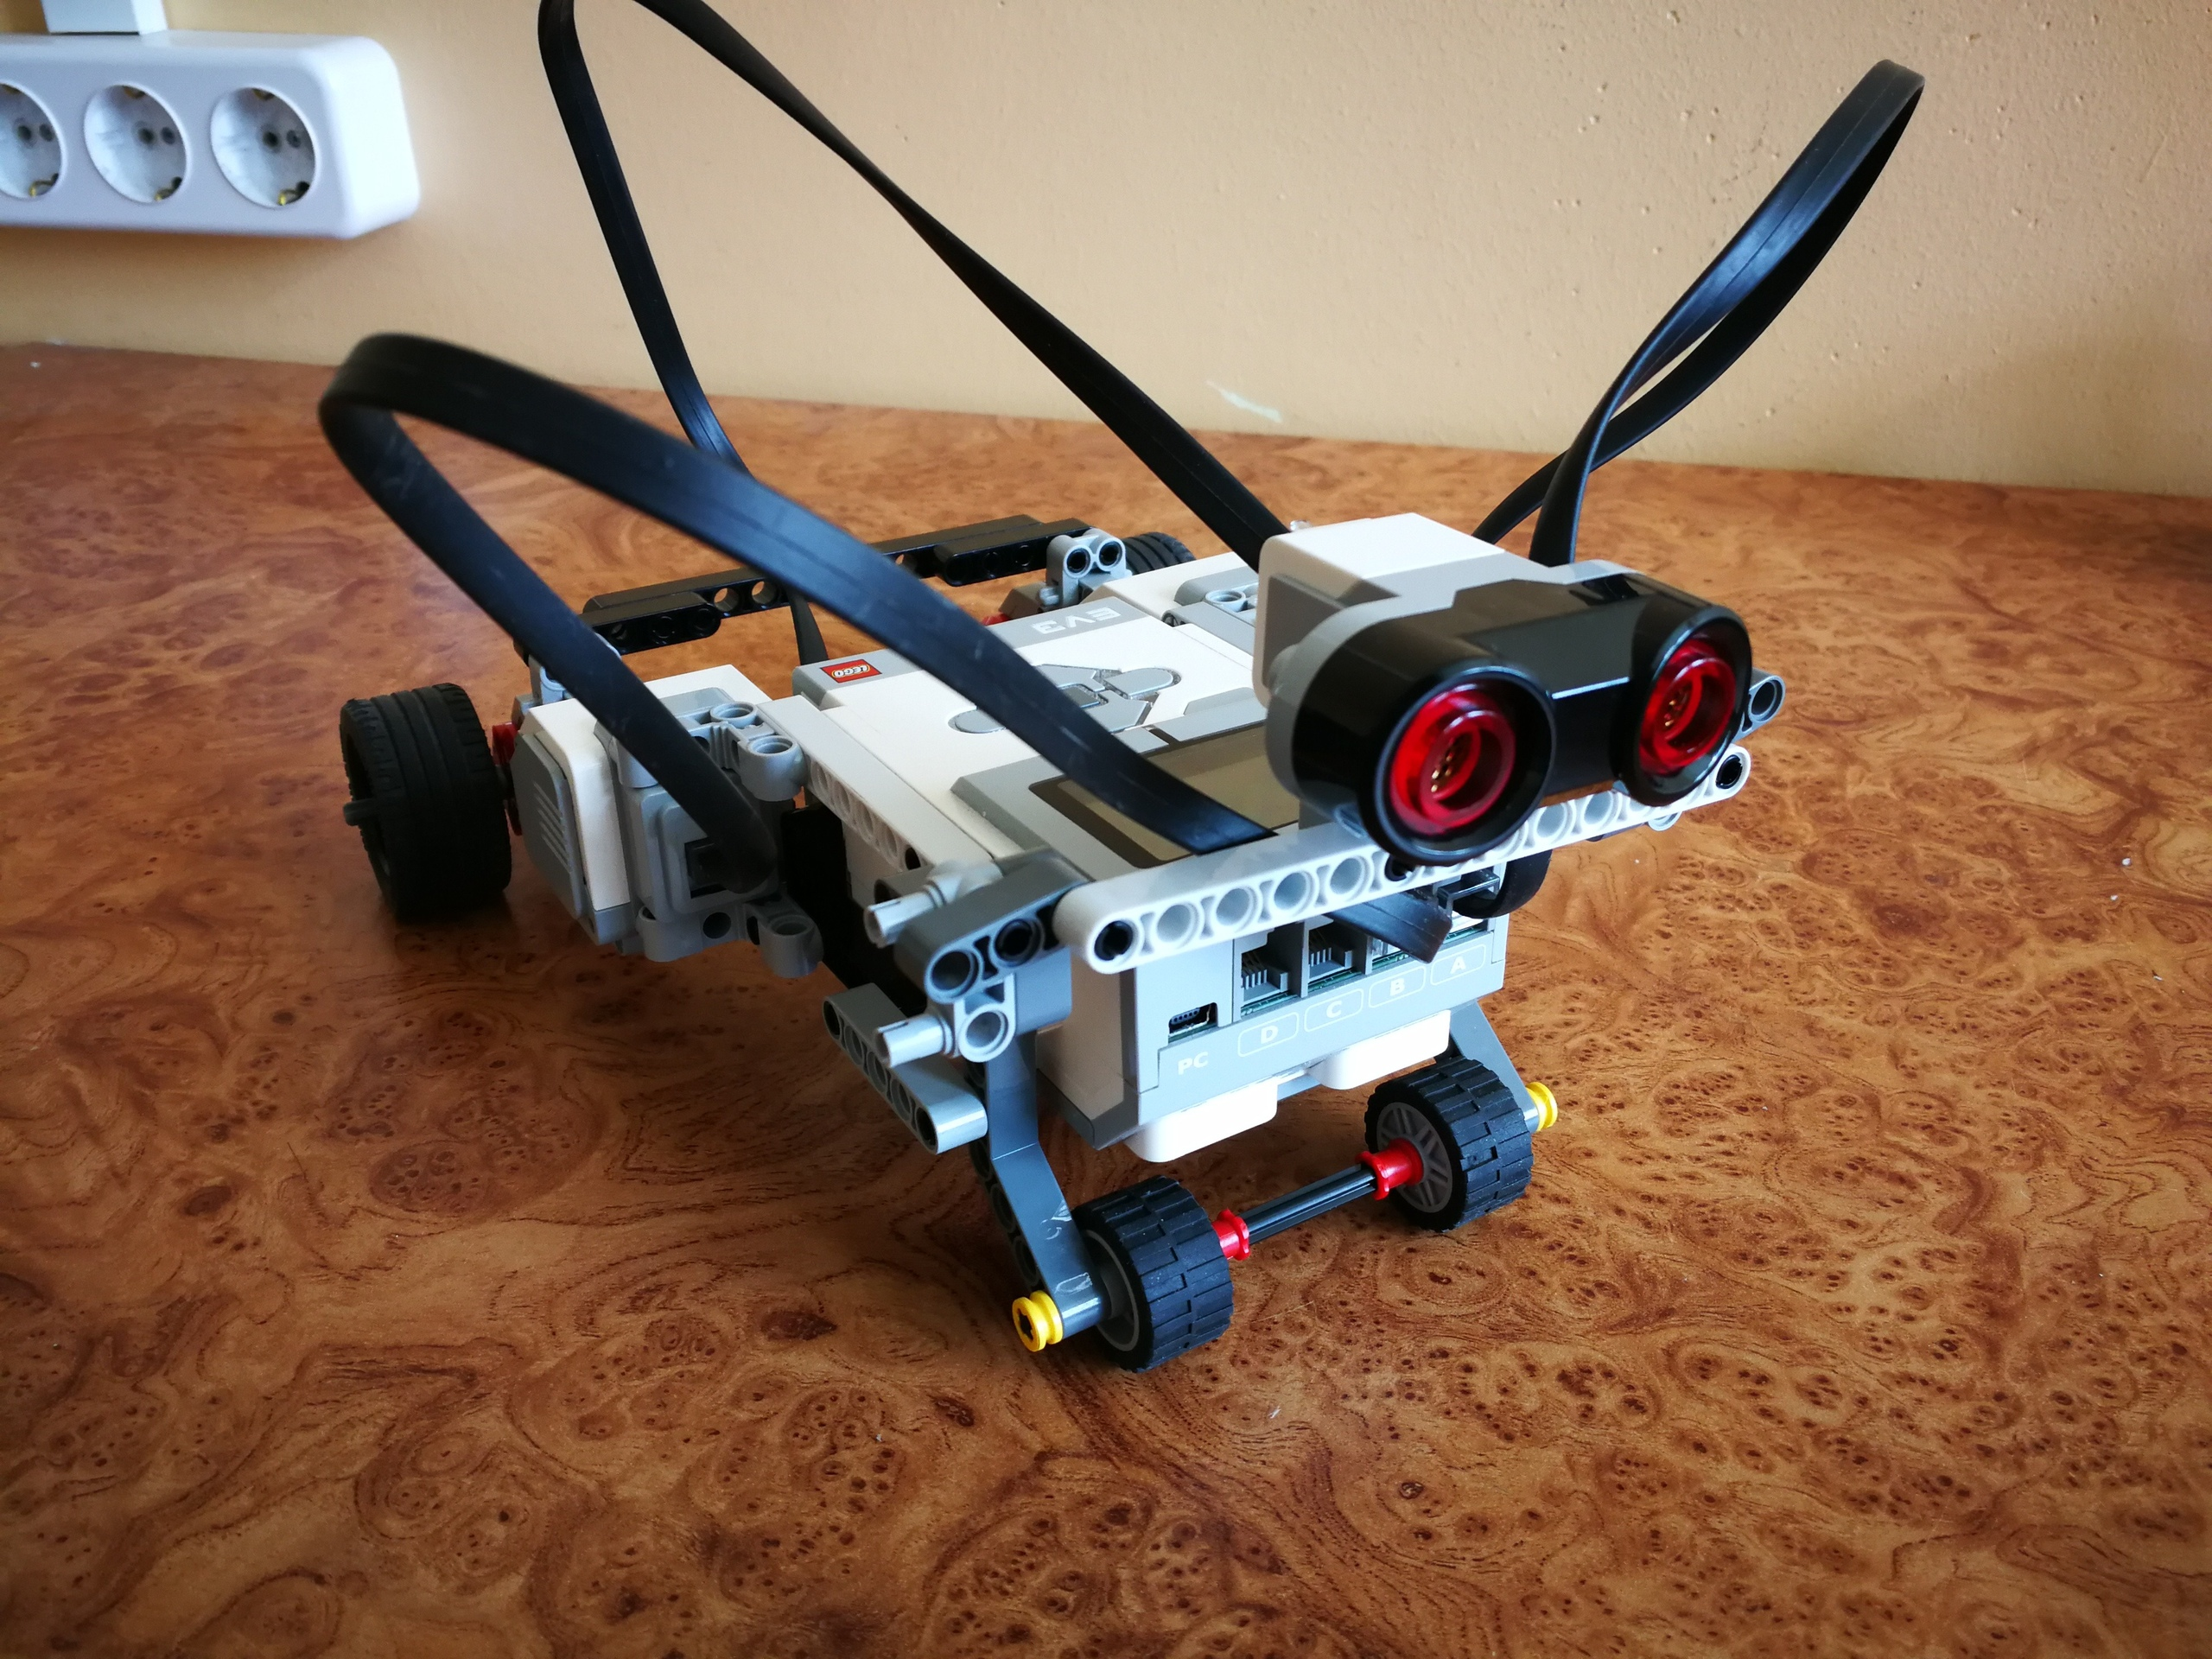
\includegraphics[height=6cm]{robocar_1_ev3.jpg}} 
			\end{minipage}
			\hfill
			\begin{minipage}[h]{0.49\linewidth}
				\center{ 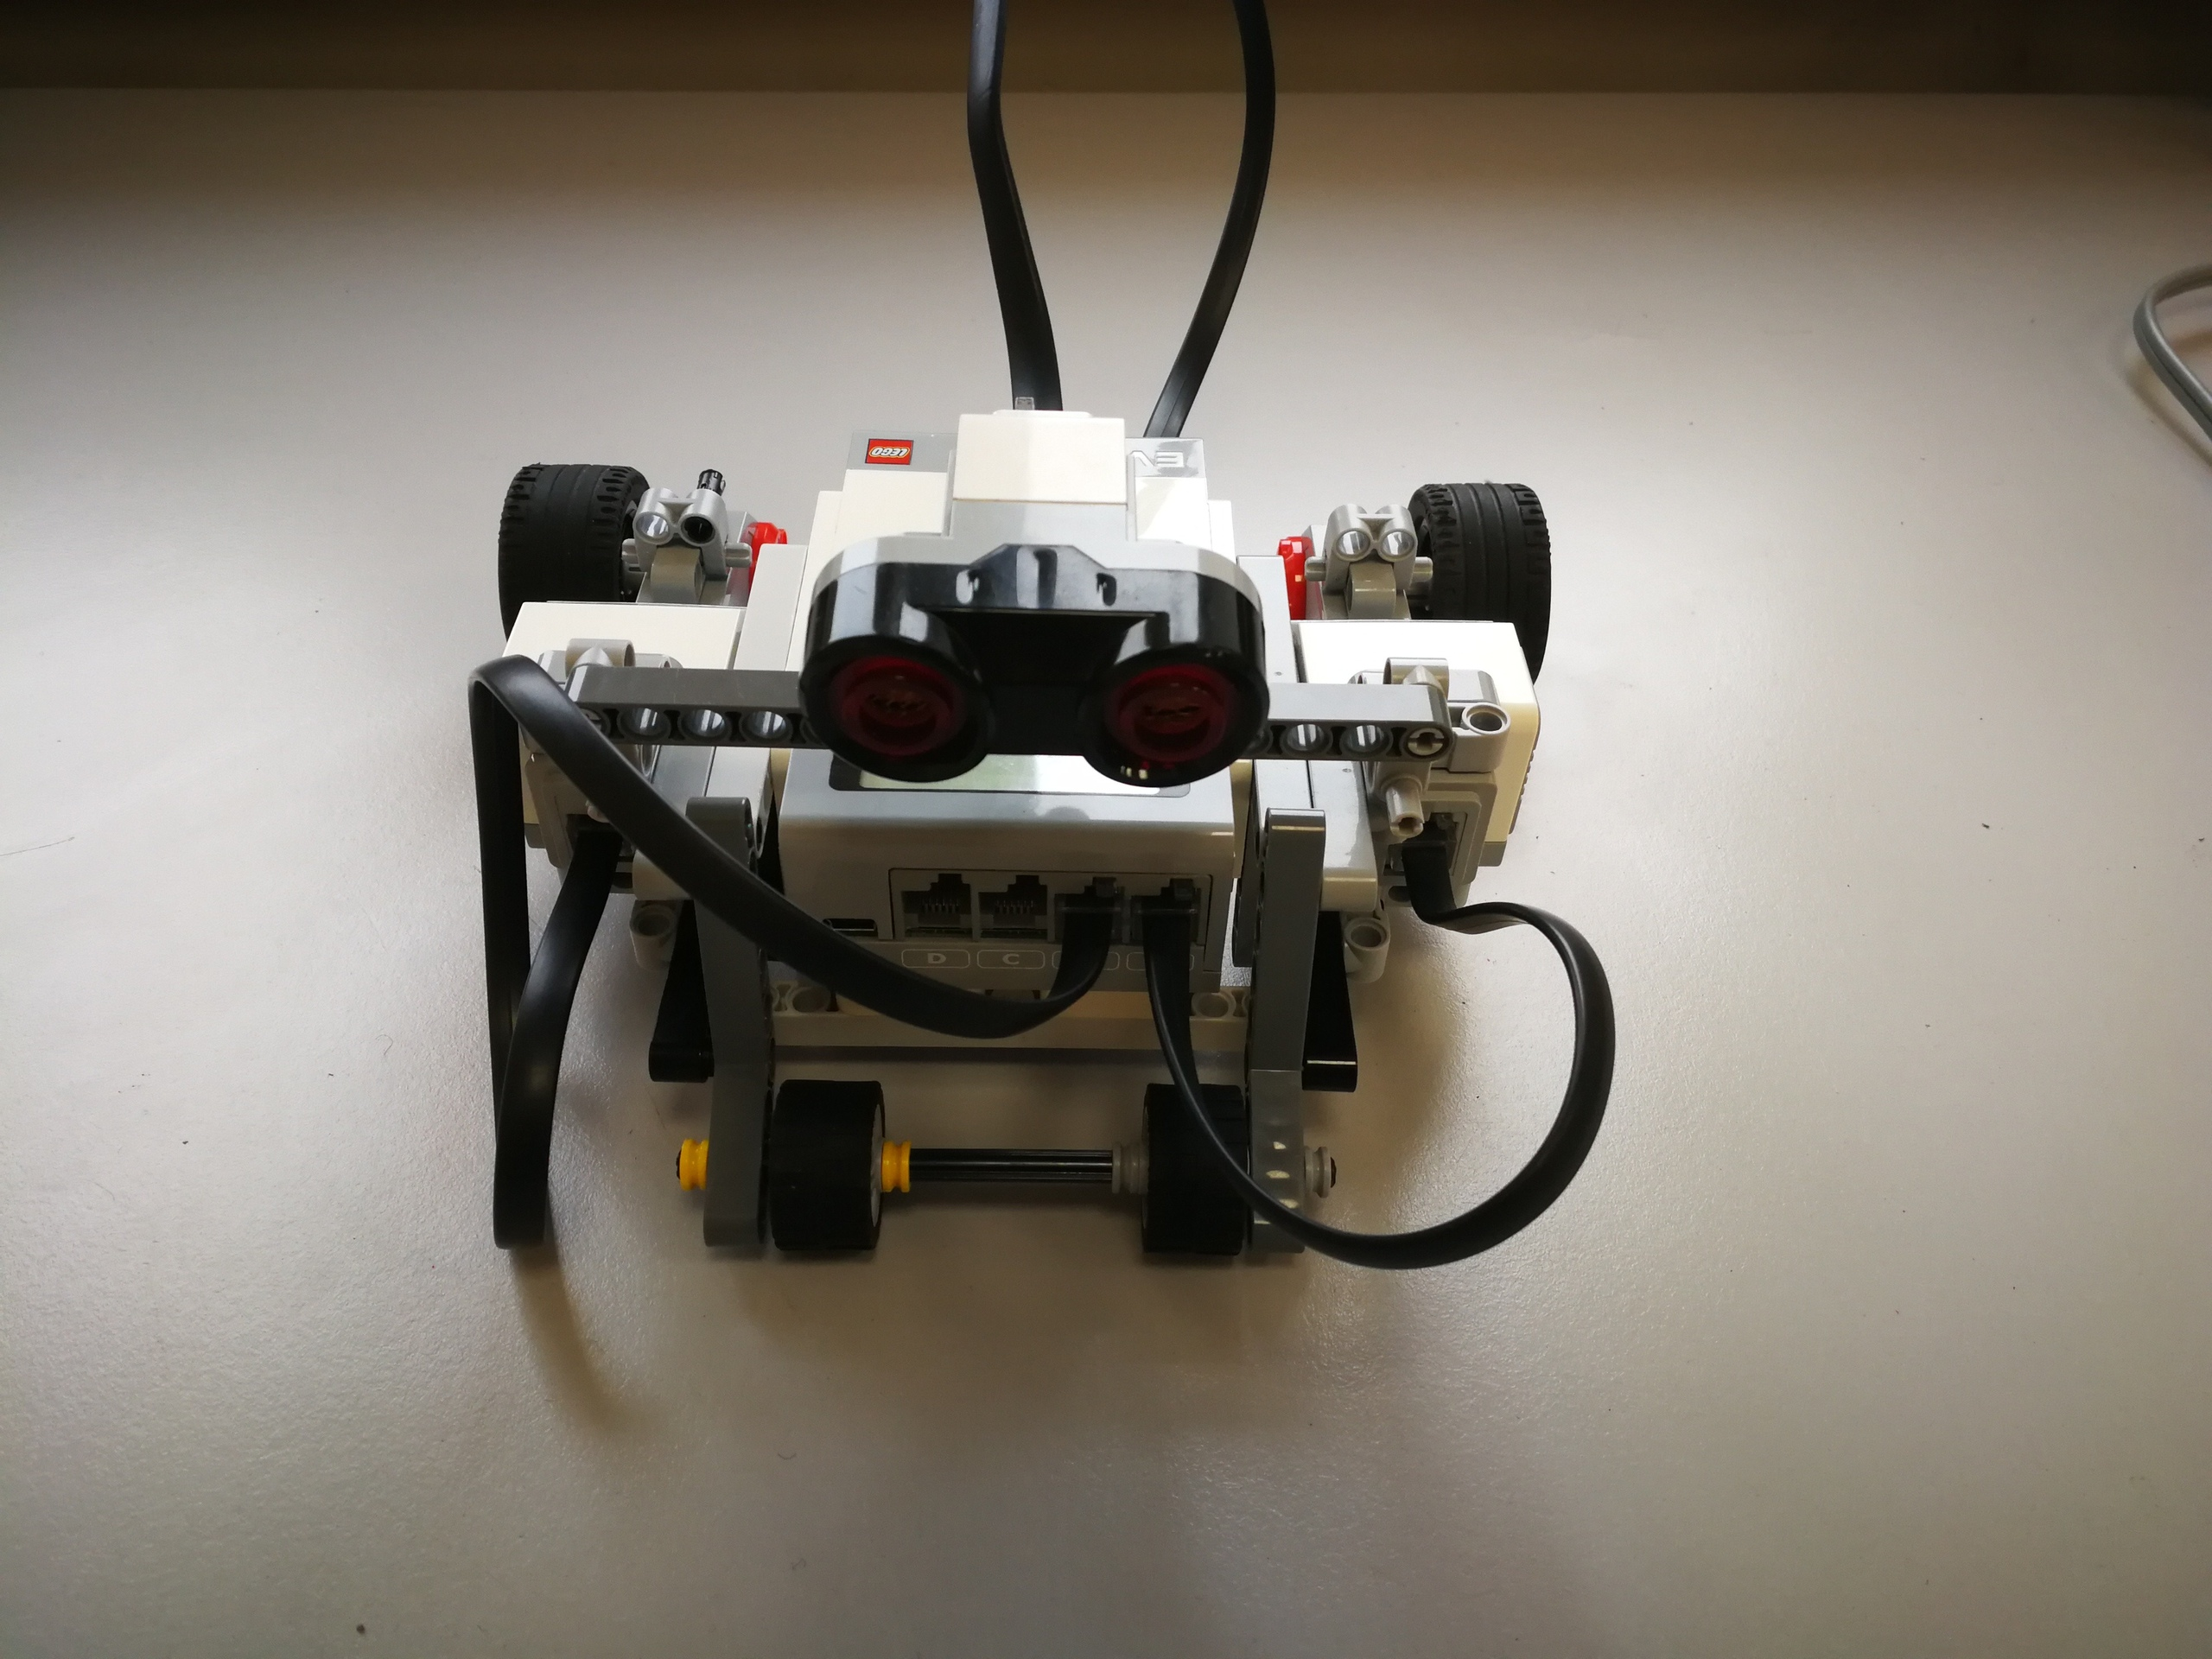
\includegraphics[height=6cm]{robocar_2_ev3.jpg}}
			\end{minipage}
			\caption{Пример требуемого робота-машинки.}
			\label{robocar}
		\end{figure}	
		\item Напишите для него программу, использующую П-регулятор, которая даст роботу умение держаться на определенном расстоянии от предстоящих ему предметов.
		Грубо говоря, если робот будет находится от препятствия на расстоянии, большем заданного, он должен будет подъехать к нему, а если слишком близко (на расстоянии, меньшем заданного), то отъехать подальше.
		Упомянутое расстояние выберите произвольно.

		Во время своей работы программа также должна записывать в текстовый файл показания, получаемые с дальномера, и соответствующие им моменты времени, прошедшего с начала работы программы.
		\item Запустите программу на выполнение и проверьте ее работоспособность, придвигая/отодвигая к/от роботу/(-а) какой-либо предмет.
		\item Используя созданный программой файл с данными постройте график зависимости показаний дальномера от времени, которая наблюдалась в ходе выше описанного эксперимента. Пример такого графика показан на рис.~\ref{distance_with_time}.
		\begin{figure}[h!]
			\centering{ 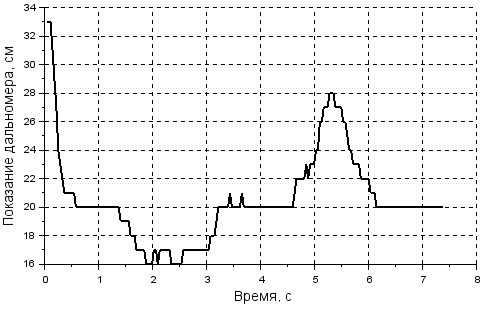
\includegraphics[scale=1.0]{distance_with_time.png} }
			\caption{Пример графика зависимости показаний дальномера от времени.}
			\label{distance_with_time}
		\end{figure}
	\end{enumerate}
\end{enumerate}
\newpage
\section{Содержание отчета}
\begin{enumerate}
\item Все графики, предусмотренные разделом <<Порядок выполнения работы>>, с указанными значениями коэффициента пропорциональности П-регулятора.
\item Исходные коды всех написанных для EV3 программ.
\item Использованная в работе схема моделирования, аналогичная той, которая представлена на рис.~\ref{struct_sheme}.
\end{enumerate}

\newpage
\section*{Приложение А\\
Использование ультразвукового датчика.}
Ультразвуковой датчик EV3, который предстоит использовать в данной работе, позволяет измерять расстояние от него до находящихся перед ним объектов. 
Принцип его работы такой же, как у обычного сонара: он посылает в заданном направление звуковую волну, измеряет время, за которое она достигнет объекта, отразится от него и придет обратно, и исходя из него определяет расстояние до препятствия.

Как и всякий другой датчик, используемый EV3, он подключается снизу главного блока~--- к одному из четырех находящихся там портов.

	\begin{figure}[h!]
		\centering{ 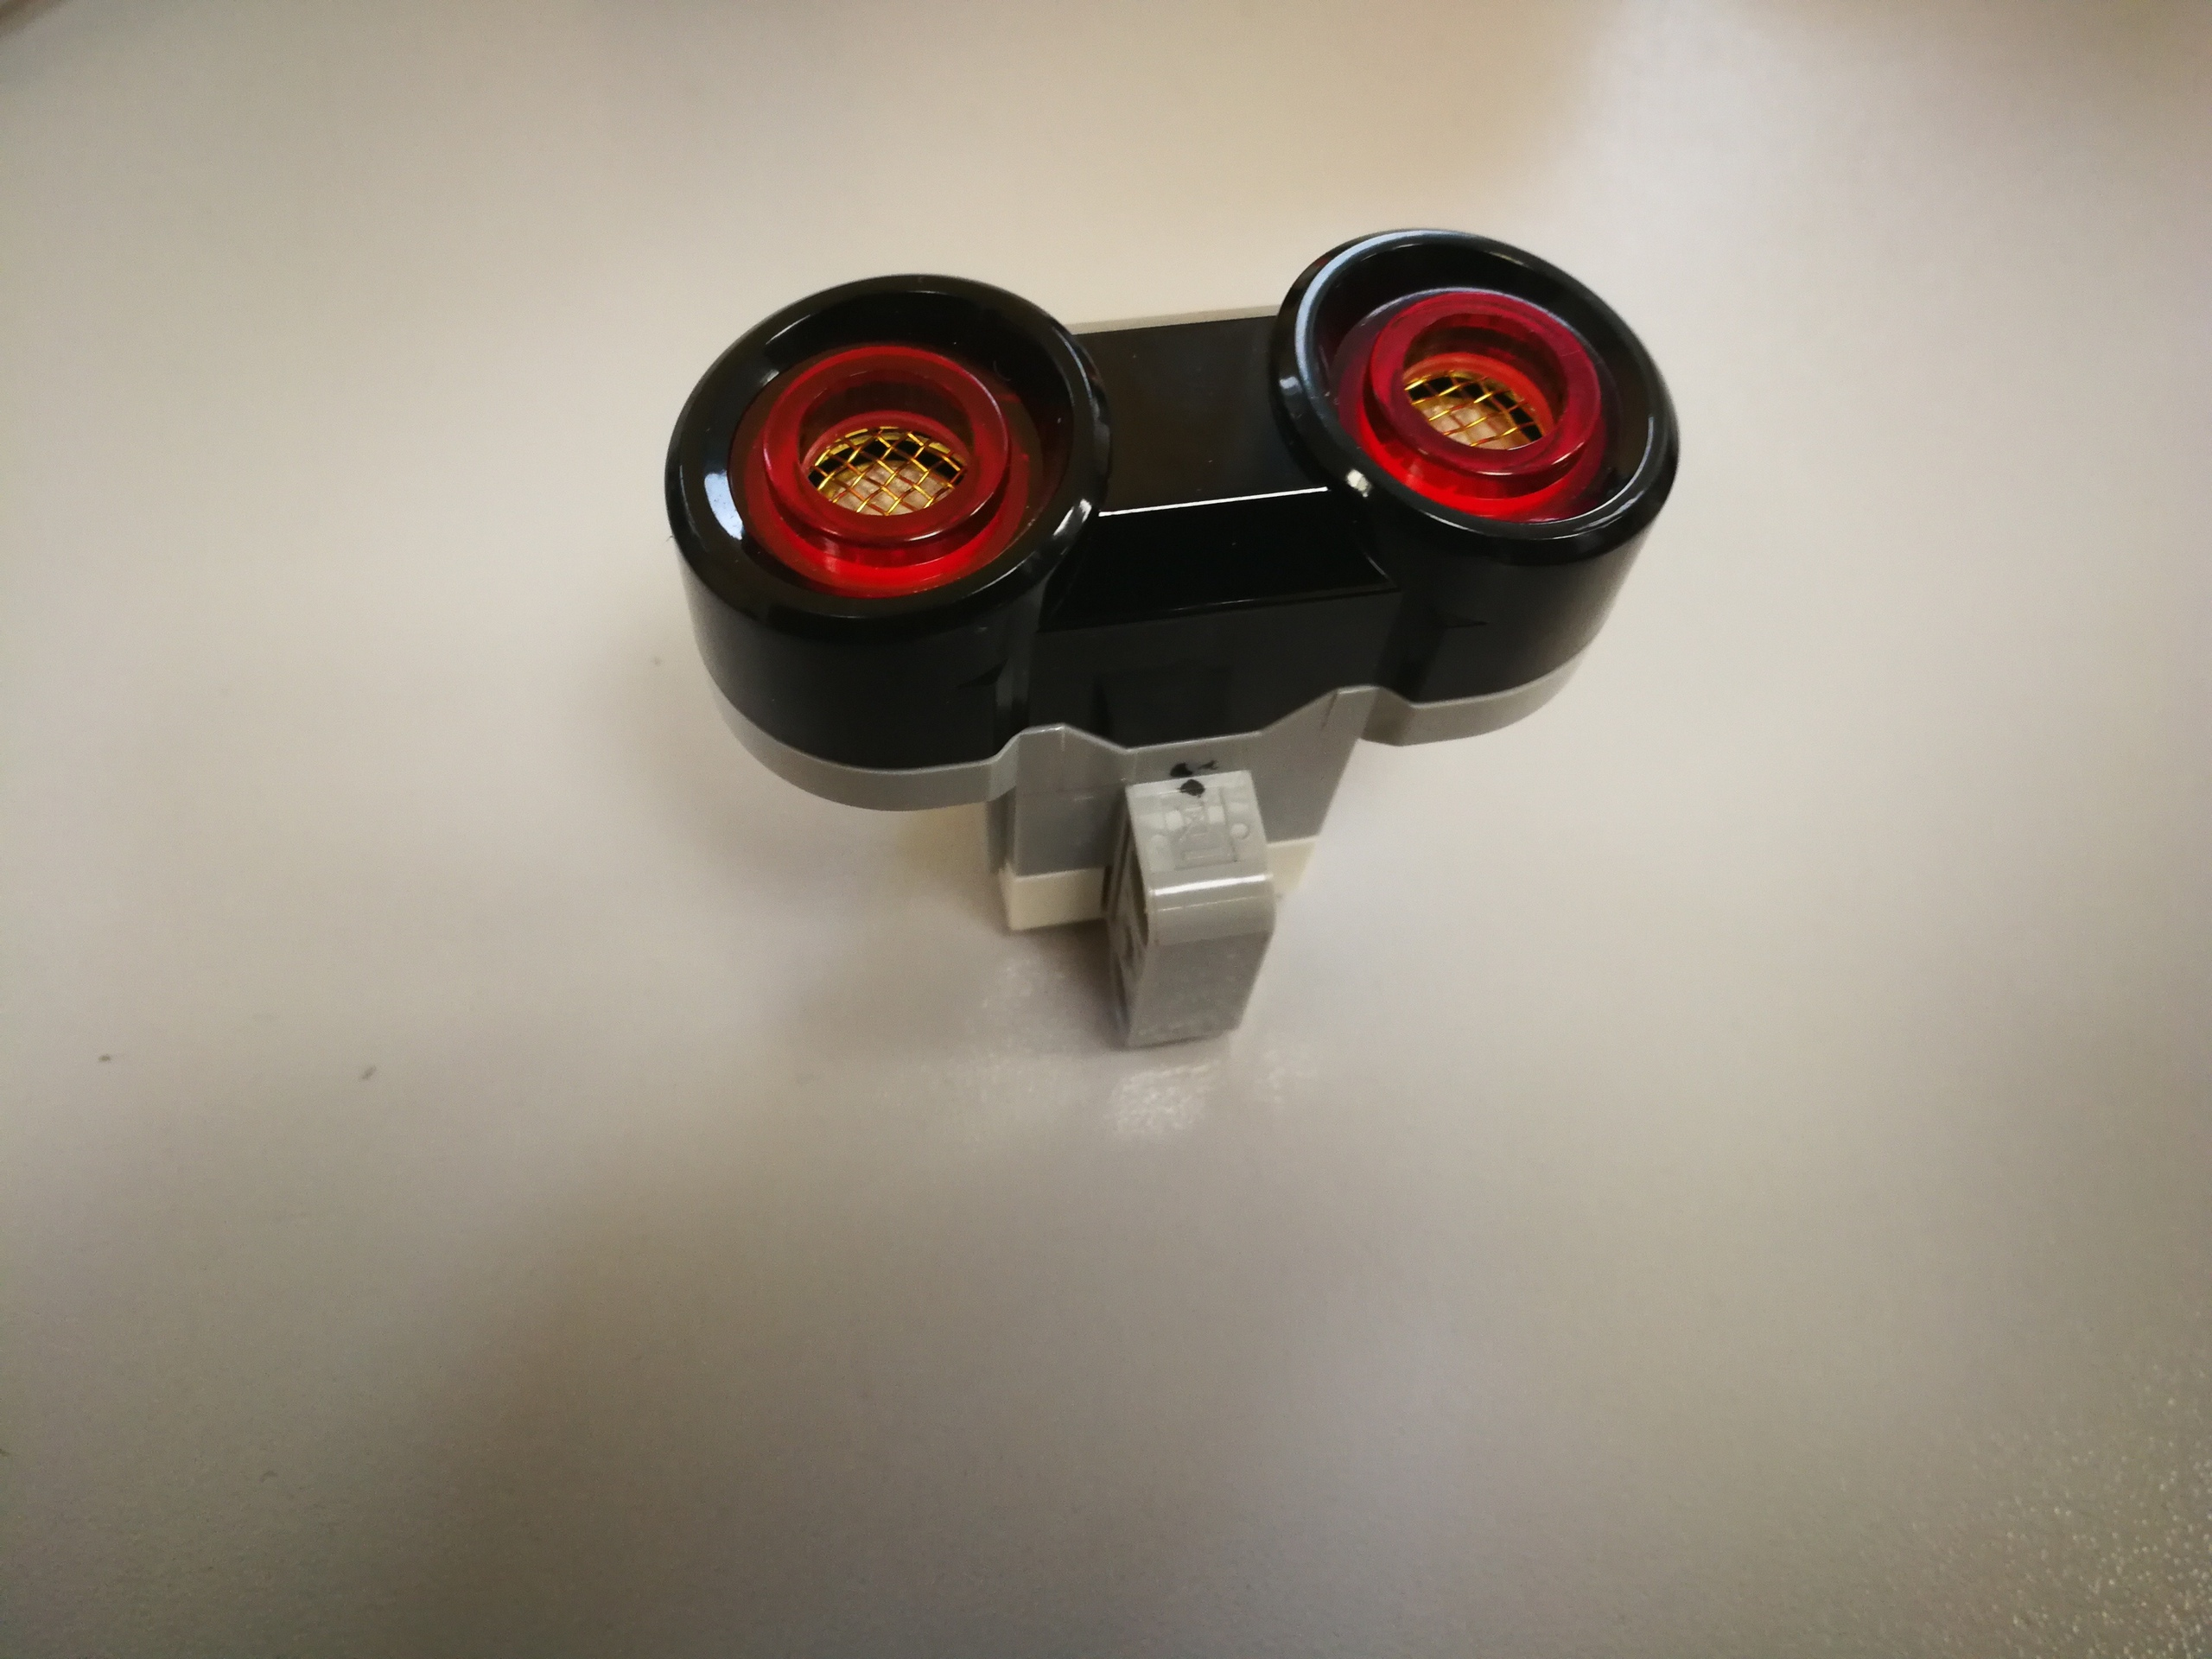
\includegraphics[scale=0.1]{ultrasonic_sensor_ev3.jpg} }
		\caption{Ультразвуковой датчик EV3.}
		\label{ultrasonic_sensor}
	\end{figure}	
	
Для того чтобы зарегистрировать ультразвуковой датчик в исполняемой программе, необходимо создать объект класса 
\verb|UltrasonicSensor(sensor_port);|.
Единственный ее аргумент, названный sensor\_port, представляет из себя номер порта, в который подключен используемый датчик, и является строкой, например \verb|"in1"|.
Получить фиксируемое датчиком расстояние (в мм) можно вызовом метода класса \verb|UtrasonicSensor.value()|.

Например, в приведенном ниже отрывке некоторой программы создается объект класса \verb|UtrasonicSensor|, соответстующий ультразуковому датчику, подключенному к порту №~1. Вызов метода \verb|mode()| с аргументом \verb|'US-DIST-CM'| устанавливает датчик на работу с метрическими единицами измерения, а затем текущее расстояние в миллиметрах, которое фиксируется ультразвуковым датчиком, подключенным к порту~№1, присваивается переменной dist:
\begin{lstlisting}
...
us_sensor = UltrasonicSensor('in1')
us_sensor.mode('US-DIST-CM')
dist = us_sensor.value() 
...
\end{lstlisting} 
\end{document}
